% Generated by Sphinx.
\def\sphinxdocclass{report}
\documentclass[letterpaper,10pt,english]{sphinxmanual}
\usepackage[utf8]{inputenc}
\DeclareUnicodeCharacter{00A0}{\nobreakspace}
\usepackage{cmap}
\usepackage[T1]{fontenc}
\usepackage{babel}
\usepackage{times}
\usepackage[Bjarne]{fncychap}
\usepackage{longtable}
\usepackage{sphinx}
\usepackage{multirow}

\addto\captionsenglish{\renewcommand{\figurename}{Fig. }}
\addto\captionsenglish{\renewcommand{\tablename}{Table }}
\floatname{literal-block}{Listing }



\title{CIVET Documentation}
\date{August 17, 2016}
\release{beta-0.9.1}
\author{Philip A. Schrodt\\Parus Analytics LLC\\Charlottesville, VA USA\\schrodt735@gmail.com}
\newcommand{\sphinxlogo}{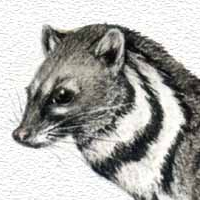
\includegraphics{civet200.png}\par}
\renewcommand{\releasename}{Release}
\makeindex

\makeatletter
\def\PYG@reset{\let\PYG@it=\relax \let\PYG@bf=\relax%
    \let\PYG@ul=\relax \let\PYG@tc=\relax%
    \let\PYG@bc=\relax \let\PYG@ff=\relax}
\def\PYG@tok#1{\csname PYG@tok@#1\endcsname}
\def\PYG@toks#1+{\ifx\relax#1\empty\else%
    \PYG@tok{#1}\expandafter\PYG@toks\fi}
\def\PYG@do#1{\PYG@bc{\PYG@tc{\PYG@ul{%
    \PYG@it{\PYG@bf{\PYG@ff{#1}}}}}}}
\def\PYG#1#2{\PYG@reset\PYG@toks#1+\relax+\PYG@do{#2}}

\expandafter\def\csname PYG@tok@gd\endcsname{\def\PYG@tc##1{\textcolor[rgb]{0.63,0.00,0.00}{##1}}}
\expandafter\def\csname PYG@tok@gu\endcsname{\let\PYG@bf=\textbf\def\PYG@tc##1{\textcolor[rgb]{0.50,0.00,0.50}{##1}}}
\expandafter\def\csname PYG@tok@gt\endcsname{\def\PYG@tc##1{\textcolor[rgb]{0.00,0.27,0.87}{##1}}}
\expandafter\def\csname PYG@tok@gs\endcsname{\let\PYG@bf=\textbf}
\expandafter\def\csname PYG@tok@gr\endcsname{\def\PYG@tc##1{\textcolor[rgb]{1.00,0.00,0.00}{##1}}}
\expandafter\def\csname PYG@tok@cm\endcsname{\let\PYG@it=\textit\def\PYG@tc##1{\textcolor[rgb]{0.25,0.50,0.56}{##1}}}
\expandafter\def\csname PYG@tok@vg\endcsname{\def\PYG@tc##1{\textcolor[rgb]{0.73,0.38,0.84}{##1}}}
\expandafter\def\csname PYG@tok@m\endcsname{\def\PYG@tc##1{\textcolor[rgb]{0.13,0.50,0.31}{##1}}}
\expandafter\def\csname PYG@tok@mh\endcsname{\def\PYG@tc##1{\textcolor[rgb]{0.13,0.50,0.31}{##1}}}
\expandafter\def\csname PYG@tok@cs\endcsname{\def\PYG@tc##1{\textcolor[rgb]{0.25,0.50,0.56}{##1}}\def\PYG@bc##1{\setlength{\fboxsep}{0pt}\colorbox[rgb]{1.00,0.94,0.94}{\strut ##1}}}
\expandafter\def\csname PYG@tok@ge\endcsname{\let\PYG@it=\textit}
\expandafter\def\csname PYG@tok@vc\endcsname{\def\PYG@tc##1{\textcolor[rgb]{0.73,0.38,0.84}{##1}}}
\expandafter\def\csname PYG@tok@il\endcsname{\def\PYG@tc##1{\textcolor[rgb]{0.13,0.50,0.31}{##1}}}
\expandafter\def\csname PYG@tok@go\endcsname{\def\PYG@tc##1{\textcolor[rgb]{0.20,0.20,0.20}{##1}}}
\expandafter\def\csname PYG@tok@cp\endcsname{\def\PYG@tc##1{\textcolor[rgb]{0.00,0.44,0.13}{##1}}}
\expandafter\def\csname PYG@tok@gi\endcsname{\def\PYG@tc##1{\textcolor[rgb]{0.00,0.63,0.00}{##1}}}
\expandafter\def\csname PYG@tok@gh\endcsname{\let\PYG@bf=\textbf\def\PYG@tc##1{\textcolor[rgb]{0.00,0.00,0.50}{##1}}}
\expandafter\def\csname PYG@tok@ni\endcsname{\let\PYG@bf=\textbf\def\PYG@tc##1{\textcolor[rgb]{0.84,0.33,0.22}{##1}}}
\expandafter\def\csname PYG@tok@nl\endcsname{\let\PYG@bf=\textbf\def\PYG@tc##1{\textcolor[rgb]{0.00,0.13,0.44}{##1}}}
\expandafter\def\csname PYG@tok@nn\endcsname{\let\PYG@bf=\textbf\def\PYG@tc##1{\textcolor[rgb]{0.05,0.52,0.71}{##1}}}
\expandafter\def\csname PYG@tok@no\endcsname{\def\PYG@tc##1{\textcolor[rgb]{0.38,0.68,0.84}{##1}}}
\expandafter\def\csname PYG@tok@na\endcsname{\def\PYG@tc##1{\textcolor[rgb]{0.25,0.44,0.63}{##1}}}
\expandafter\def\csname PYG@tok@nb\endcsname{\def\PYG@tc##1{\textcolor[rgb]{0.00,0.44,0.13}{##1}}}
\expandafter\def\csname PYG@tok@nc\endcsname{\let\PYG@bf=\textbf\def\PYG@tc##1{\textcolor[rgb]{0.05,0.52,0.71}{##1}}}
\expandafter\def\csname PYG@tok@nd\endcsname{\let\PYG@bf=\textbf\def\PYG@tc##1{\textcolor[rgb]{0.33,0.33,0.33}{##1}}}
\expandafter\def\csname PYG@tok@ne\endcsname{\def\PYG@tc##1{\textcolor[rgb]{0.00,0.44,0.13}{##1}}}
\expandafter\def\csname PYG@tok@nf\endcsname{\def\PYG@tc##1{\textcolor[rgb]{0.02,0.16,0.49}{##1}}}
\expandafter\def\csname PYG@tok@si\endcsname{\let\PYG@it=\textit\def\PYG@tc##1{\textcolor[rgb]{0.44,0.63,0.82}{##1}}}
\expandafter\def\csname PYG@tok@s2\endcsname{\def\PYG@tc##1{\textcolor[rgb]{0.25,0.44,0.63}{##1}}}
\expandafter\def\csname PYG@tok@vi\endcsname{\def\PYG@tc##1{\textcolor[rgb]{0.73,0.38,0.84}{##1}}}
\expandafter\def\csname PYG@tok@nt\endcsname{\let\PYG@bf=\textbf\def\PYG@tc##1{\textcolor[rgb]{0.02,0.16,0.45}{##1}}}
\expandafter\def\csname PYG@tok@nv\endcsname{\def\PYG@tc##1{\textcolor[rgb]{0.73,0.38,0.84}{##1}}}
\expandafter\def\csname PYG@tok@s1\endcsname{\def\PYG@tc##1{\textcolor[rgb]{0.25,0.44,0.63}{##1}}}
\expandafter\def\csname PYG@tok@gp\endcsname{\let\PYG@bf=\textbf\def\PYG@tc##1{\textcolor[rgb]{0.78,0.36,0.04}{##1}}}
\expandafter\def\csname PYG@tok@sh\endcsname{\def\PYG@tc##1{\textcolor[rgb]{0.25,0.44,0.63}{##1}}}
\expandafter\def\csname PYG@tok@ow\endcsname{\let\PYG@bf=\textbf\def\PYG@tc##1{\textcolor[rgb]{0.00,0.44,0.13}{##1}}}
\expandafter\def\csname PYG@tok@sx\endcsname{\def\PYG@tc##1{\textcolor[rgb]{0.78,0.36,0.04}{##1}}}
\expandafter\def\csname PYG@tok@bp\endcsname{\def\PYG@tc##1{\textcolor[rgb]{0.00,0.44,0.13}{##1}}}
\expandafter\def\csname PYG@tok@c1\endcsname{\let\PYG@it=\textit\def\PYG@tc##1{\textcolor[rgb]{0.25,0.50,0.56}{##1}}}
\expandafter\def\csname PYG@tok@kc\endcsname{\let\PYG@bf=\textbf\def\PYG@tc##1{\textcolor[rgb]{0.00,0.44,0.13}{##1}}}
\expandafter\def\csname PYG@tok@c\endcsname{\let\PYG@it=\textit\def\PYG@tc##1{\textcolor[rgb]{0.25,0.50,0.56}{##1}}}
\expandafter\def\csname PYG@tok@mf\endcsname{\def\PYG@tc##1{\textcolor[rgb]{0.13,0.50,0.31}{##1}}}
\expandafter\def\csname PYG@tok@err\endcsname{\def\PYG@bc##1{\setlength{\fboxsep}{0pt}\fcolorbox[rgb]{1.00,0.00,0.00}{1,1,1}{\strut ##1}}}
\expandafter\def\csname PYG@tok@mb\endcsname{\def\PYG@tc##1{\textcolor[rgb]{0.13,0.50,0.31}{##1}}}
\expandafter\def\csname PYG@tok@ss\endcsname{\def\PYG@tc##1{\textcolor[rgb]{0.32,0.47,0.09}{##1}}}
\expandafter\def\csname PYG@tok@sr\endcsname{\def\PYG@tc##1{\textcolor[rgb]{0.14,0.33,0.53}{##1}}}
\expandafter\def\csname PYG@tok@mo\endcsname{\def\PYG@tc##1{\textcolor[rgb]{0.13,0.50,0.31}{##1}}}
\expandafter\def\csname PYG@tok@kd\endcsname{\let\PYG@bf=\textbf\def\PYG@tc##1{\textcolor[rgb]{0.00,0.44,0.13}{##1}}}
\expandafter\def\csname PYG@tok@mi\endcsname{\def\PYG@tc##1{\textcolor[rgb]{0.13,0.50,0.31}{##1}}}
\expandafter\def\csname PYG@tok@kn\endcsname{\let\PYG@bf=\textbf\def\PYG@tc##1{\textcolor[rgb]{0.00,0.44,0.13}{##1}}}
\expandafter\def\csname PYG@tok@o\endcsname{\def\PYG@tc##1{\textcolor[rgb]{0.40,0.40,0.40}{##1}}}
\expandafter\def\csname PYG@tok@kr\endcsname{\let\PYG@bf=\textbf\def\PYG@tc##1{\textcolor[rgb]{0.00,0.44,0.13}{##1}}}
\expandafter\def\csname PYG@tok@s\endcsname{\def\PYG@tc##1{\textcolor[rgb]{0.25,0.44,0.63}{##1}}}
\expandafter\def\csname PYG@tok@kp\endcsname{\def\PYG@tc##1{\textcolor[rgb]{0.00,0.44,0.13}{##1}}}
\expandafter\def\csname PYG@tok@w\endcsname{\def\PYG@tc##1{\textcolor[rgb]{0.73,0.73,0.73}{##1}}}
\expandafter\def\csname PYG@tok@kt\endcsname{\def\PYG@tc##1{\textcolor[rgb]{0.56,0.13,0.00}{##1}}}
\expandafter\def\csname PYG@tok@sc\endcsname{\def\PYG@tc##1{\textcolor[rgb]{0.25,0.44,0.63}{##1}}}
\expandafter\def\csname PYG@tok@sb\endcsname{\def\PYG@tc##1{\textcolor[rgb]{0.25,0.44,0.63}{##1}}}
\expandafter\def\csname PYG@tok@k\endcsname{\let\PYG@bf=\textbf\def\PYG@tc##1{\textcolor[rgb]{0.00,0.44,0.13}{##1}}}
\expandafter\def\csname PYG@tok@se\endcsname{\let\PYG@bf=\textbf\def\PYG@tc##1{\textcolor[rgb]{0.25,0.44,0.63}{##1}}}
\expandafter\def\csname PYG@tok@sd\endcsname{\let\PYG@it=\textit\def\PYG@tc##1{\textcolor[rgb]{0.25,0.44,0.63}{##1}}}

\def\PYGZbs{\char`\\}
\def\PYGZus{\char`\_}
\def\PYGZob{\char`\{}
\def\PYGZcb{\char`\}}
\def\PYGZca{\char`\^}
\def\PYGZam{\char`\&}
\def\PYGZlt{\char`\<}
\def\PYGZgt{\char`\>}
\def\PYGZsh{\char`\#}
\def\PYGZpc{\char`\%}
\def\PYGZdl{\char`\$}
\def\PYGZhy{\char`\-}
\def\PYGZsq{\char`\'}
\def\PYGZdq{\char`\"}
\def\PYGZti{\char`\~}
% for compatibility with earlier versions
\def\PYGZat{@}
\def\PYGZlb{[}
\def\PYGZrb{]}
\makeatother

\renewcommand\PYGZsq{\textquotesingle}

\begin{document}

\maketitle
\tableofcontents
\phantomsection\label{index::doc}\section*{Preface}
This is the documentation for the CIVET—Contentious Incident Variable Entry Template—data entry system.
CIVET was developed under the NSF-sponsored project titled “A Method for Leveraging Public Information
Sources for Social Science Research” which is creating tools to improve the efficiency of data generation
in the social sciences, with an initial focus on coding event data in the domain of contentious politics.

The system is deployed as a \href{https://www.djangoproject.com/start/overview/}{Django} application;
it should be possible to get this working by installing Django on a local machine and copying the directory \code{djcivet\_site}.

We are very interested in feedback on this system, including any bugs
you encounter (please let us know what operating system (e.g. Windows,
OS-X) and browser (e.g. FireFox, Explorer, Chrome) you were using),
aspects of the manual that are unclear (and features that appear too
complex), and additional features that would be useful. Please send any
suggestions to \href{mailto:schrodt735@gmail.com}{schrodt735@gmail.com}.

\href{https://github.com/civet-software}{Link to} the software on GitHub
\section*{Acknowledgements}
The development of CIVET is funded by the U.S. National Science Foundation Office of Multidisciplinary Activities
in the Directorate for Social, Behavioral \& Economic Sciences, Award 1338470 and the \href{http://www.odum.unc.edu/odum/home2.jsp}{Odum Institute} at the University of North Carolina at Chapel Hill with additional assistance from \href{http://parusanalytics.com/}{Parus Analytics}. This documentation is licensed under a Creative Commons Attribution-NonCommercial 4.0 International License; CIVET is open source and under the MIT license.
Any opinions, findings, and conclusions or recommendations expressed in this material are those of the authors
and do not necessarily reflect the views of the National Science Foundation.




\chapter{Introduction}
\label{intro:introduction}\label{intro::doc}\label{intro:id1}
This is the documentation for
CIVET \footnote{
\href{http://en.wikipedia.org/wiki/CIVET}{http://en.wikipedia.org/wiki/CIVET}
}—Contentious Incident Variable Entry Template—customizable
data entry system. CIVET was developed by the NSF-sponsored project
titled “A Method for Leveraging Public Information Sources for Social
Science Research” which is creating tools to improve the efficiency of
data generation in the social sciences. The project had an initial focus
on coding event data in the domain of contentious politics, but we
expect that these tools will be relevant in a number of data-generation
domains.

The core objective of CIVET is to provide a reasonably simple—yes,
simple—set of commands that will allow a user to set up a web-based
coding environment without the need to master the likes of HTML, CSS and
Javascript. As currently implemented, the system is a rather ugly
prototype; it will also be evolving as we add additional elements.
Nonetheless, the system should now be useable for coding.

CIVET is implemented in the widely-used and well documented
Python-based Django system \footnote{
An earlier prototype was implemented in the \code{Flask} framework: see
Appendix 4
} which is widely available on various
cloud platforms: a rather extended list of “Django-friendly” hosting
services can be found at
\begin{quote}

\href{https://code.djangoproject.com/wiki/DjangoFriendlyWebHosts}{https://code.djangoproject.com/wiki/DjangoFriendlyWebHosts}
\end{quote}

The complete CIVET code is licensed as open source under the MIT
license and provided on GitHub at \href{https://github.com/civet-software}{https://github.com/civet-software} .

CIVET currently has two modes:
\begin{description}
\item[{\textbf{Coding form template:}}] \leavevmode
This is a template-based for setting up a web-based coding form
which implements several of the common HTML data entry formats and
exports the resulting data as a tab-delimited text file. This is
fully functional and should be useable for small projects.

\item[{\textbf{Text annotation/extraction:}}] \leavevmode
This uses CIVET “workspaces” which combine related texts, their
metadata, and the coding form. Workspaces allow for manual and
automated text annotation, then the ability to extract various types
of information into the fields of a coding form.

\end{description}


\section{Program Navigation Placeholders}
\label{intro:program-navigation-placeholders}
CIVET is still under development and not all of the options have
been fully implemented. If you see a page with a message of the form
\begin{quote}

\code{The option {[}something{]} has yet to be implemented. Use the back arrow in your browser to return to the previous screen.}
\end{quote}

you have encountered one of those options: as noted, just use the “Back”
option in your browser to return to the previous screen. These are primarily
in the “Workspace Management” papge.


\section{Status of the Program: 31 August 2015}
\label{intro:status-of-the-program-31-august-2015}
The NSF funding for the project ended on this date. At this point, all of
the documented features of the program should be working except as
noted above. However, we are just beginning the process of
operational field testing and it is likely—which is to say, inevitable—
that some additional bugs will be found, hence this is still considered
“Beta-0.9” rather than “1.0.” We currently have two field tests underway,
and are hoping to get some additional ones going, and will be posting
bug fixes to GitHub promptly as these appear and are resolved.

At present, we have not developed any software for generating the
workspace files, though we expect to have at least a couple programs
available in the next few months. The problem here is that identifying
the various metadata and components in a set of texts is highly
specific to the text source, and to date we've not found general
solutions for this. As noted in the final chapter of this document,
over the next year or so we will be seeking additional funding for
tool development for these “front-end” tasks, though given the very
slow pace of the public funding cycle, this is unlikely to occur until
late in 2016 at the earliest. In the meantime, we will be leveraging
tools developed in existing projects and, of course, would very
much appreciate the contribution of any ancillary tools that the user
community develops, particularly for common sources such as Lexis-Nexis,
Factiva, ProQuest, LDC Gigaword, and various news feeds and social
media.


\section{Status of the Program: August 2016}
\label{intro:status-of-the-program-august-2016}
Over the past year, CIVET has been used in two projects, though both with
my assistance in generating the YAML files and with some additional
customization, much of which has been incorporated into the general
system.

To my knowledge, however—and if you know of some project using this,
please let me know—it has not been used for the originally intended
purpose of providing a platform which would allow someone with relatively
limited programming knowledge to create a web-based form. I suspect this
is due to one or more of the following factors:
\begin{itemize}
\item {} 
The process of getting Django installed, while thoroughly documented,
apparently can require some experimentation and tweaking. That
said, one of the projects decided to install Django on laptops
used by the coders rather than through a server: this
allowed the coders to work anywhere.

\item {} 
When using workspaces, which allow access to the most sophisticated
parts of the system, the texts must be converted to the YAML
format, a task for which I've yet to see a general solution and
almost certainly requires Python, perl or Java programming skills

\item {} 
Realistically, there are only a small number of new projects starting in any given
year which are sufficiently large that existing tools such as
spreadsheets or Google Forms are inadequate. And many of those,
of course, will have resources to directly develop customized
pages rather than working within the constraints of CIVET

\end{itemize}

So, this is essentially just an open-source version of a codebase that
I can customize to generate coding forms. Which I'm realizing is
probably pretty much what about 95\% of open-source projects are, though
that still gives the client a whole lot more knowledge and power than
they have with a proprietary system, even if they never change a line
of code. Whatever.

Some random observations from those two deployments:
\begin{itemize}
\item {} 
Additional customization of the code has gone quite smoothly, even
allowing for the inevitable decay of my comprehension of the
system. Granted, even when I've forgotten the details of the code
I'm still working with my programming idioms, but it does seem like as a
base, this is quite solid. The same can be said for the YAML
workspace format.

\item {} 
Neither of the two installations made any use of the manual
annotation, and in the second, the \code{NEVER\_ANNOTATE} option was
added to bypass this entirely: annotation is either handled
automatically using vocabulary files, or directly putting the
HTML into the YAML files.

\item {} 
More generally, though completely expected, the deployment have
generated a number of interesting ideas for new features that
did not emerge in the abstract design phase. I've also left
in some custom code—commented-out or otherwise deactivated—
that could be used for examples of further possible extensions.

\item {} 
On two occasions over the past year there were changes to
Django that required minor changes—one or two lines of code—
to CIVET in order to keep it running. Unsurprisingly, we have
also found that Django is more likely to be fully compatible
with up-to-date hardware
and operating systems: in particular, one project ran into some
issues running it on some old copies of Windows. Once again, this is
less of a turn-key system than I'd hoped.

\end{itemize}


\section{Documentation}
\label{intro:documentation}
Documentation is maintained using the \href{http://http://sphinx-doc.org/}{Sphinx} system, which provides both an
\href{http://civet.parusanalytics.com/civetdocs/index.html}{on-line version} and a reasonably-well-formatted PDF version. There
are links to both of these compiled versions on the home page; the \code{.rst} source texts for the documentation are in the
directory \emph{djcivet\_site/docs}. That directory contains a Sphinx \emph{Makefile} so revisions can be compiled using the standard
command \code{make html latexpdf}.

The on-line documentation currently resides at the site \href{http://civet.parusanalytics.com/civetdocs/}{http://civet.parusanalytics.com/civetdocs/}; \footnote{
This is a bug, not a feature: there is presumably a way of accessing these at \emph{djcivet\_site/docs/\_build/html/}, or
somewhere else within the \emph{djcivet\_site/} directory
in a manner that has them correctly rendered, but I haven't figured it out yet. Fixes are welcome.
} a PDF version can
be downloaded by clicking the \code{Download PDF} link on the home page. \footnote{
This is handled in \code{views.download\_pdfdocs()}: it first looks for the PDF version of the documentation in
\emph{docs/\_build/latex/civetdoc.pdf}, which is where the most current version is likely to be located when the
documentation was produced using the \code{make latexpdf} command in the \emph{docs/} directory. If that isn't present,
it checks the \emph{/static/} directory: this can be used in deployments in order to avoid uploading  \emph{docs/}. If neither
is available, it gets the copy posted at \href{http://civet.parusanalytics.com/}{http://civet.parusanalytics.com/}, which may or may not correspond exactly to the
version being used depending on what modifications have been made. The command \code{make movepdf} will copy \emph{civetdoc.pdf} from
\emph{\_build/latex} to \emph{/static/}
}


\chapter{Installing CIVET}
\label{installing:installing-civet}\label{installing::doc}
To date we’ve only installed the system on Macintosh computers (OS-X), though
the only difference between a Macintosh installation and other
installations should be the installation of the Django system.

On Macintoshes running OS-X 9 and 10, the required Python 2.7 comes
pre-installed. The \code{pip} installation program may also be
pre-installed—I’m having trouble determining this from the Web, and
forget whether I had to install it when I last upgraded—but if not,
install that.
\begin{enumerate}
\item {} 
In the Terminal, run \code{sudo pip install Django}: you will need
administrative access to do this.

\item {} 
Download the CIVET system from
\href{https://github.com/civet-software/CIVET-Django}{https://github.com/civet-software/CIVET-Django}, unzip the folder and
put it wherever you would like

\item {} 
In the Terminal, change the directory so that you are in the folder
\emph{Django\_CIVET/djcivet\_site}

\item {} 
In the Terminal, enter \code{python manage.py runserver}

\item {} 
In a browser, enter the URL \href{http://127.0.0.1:8000}{http://127.0.0.1:8000}

\end{enumerate}

At this point you should see the CIVET home screen \footnote{
If you see a log-in page requesting a user name and password, the log-in requirement
has been activated: see the “Authentication” chapter for details on how to use
(or deactivate) this.
}
\begin{figure}[htbp]
\centering

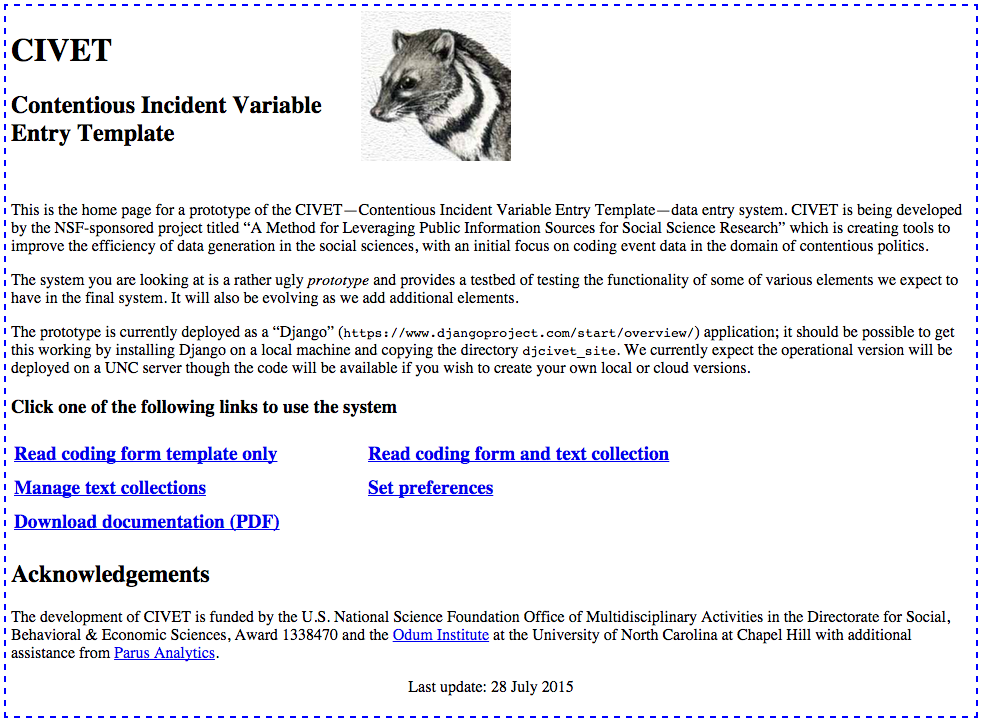
\includegraphics[width=1.000\linewidth]{civethome.png}
\end{figure}


\section{Modifying the default installation}
\label{installing:modifying-the-default-installation}
Because CIVET is still in beta, the version on GitHub is the one being used for
development. To deploy the system for active coding, you will probably want
to make the following changes:
\begin{enumerate}
\item {} \begin{description}
\item[{In the file \emph{djcivet\_site/djcivet\_site/settings.py}, set \code{DEBUG = False}.}] \leavevmode
This will

It is appropriate to note the \href{https://docs.djangoproject.com/en/1.8/ref/settings/}{Django documentation advice}
on this:

\begin{Verbatim}[commandchars=\\\{\}]
Never deploy a site into production with DEBUG turned on.

Did you catch that? NEVER deploy a site into production with DEBUG turned on.
\end{Verbatim}

As the Django documentation discusses in detail, with \code{DEBUG = True} any
errors will generate an error page containing extensive internal detail
about your site. With \code{DEBUG = False}, the user just sees a \code{Page not found}
error.

\end{description}

\end{enumerate}


\chapter{Authentication}
\label{authentication:authentication}\label{authentication::doc}
Django famously includes, ``out of the box'', a very robust system for handling user authentication and permissions. Except
for a few minor modifications such as changing the web page headings and providing vaguely informative messages for log-in
failures, CIVET simply implements the default version of this, so you can be guided the instructions at
\href{https://docs.djangoproject.com/en/1.8/topics/auth/}{https://docs.djangoproject.com/en/1.8/topics/auth/}.

Authentication is controlled by the \emph{civet\_settings.py} global variable \code{REQUIRE\_LOGIN}. By default, this is set to
\code{True} when \code{PRODUCTION\_MODE = True} and \code{False} otherwise. If you enter the name of the site without any additional
arguments, the program will go to a login page when \code{civet\_settings.REQUIRE\_LOGIN = True}; otherwise it will go
directly to the home page.
Attempting to access the home page when \code{REQUIRE\_LOGIN = True} without a login will redirect to the login page.


\section{Creating a superuser}
\label{authentication:creating-a-superuser}
To keep things simple, CIVET handles the administration of users through the controls available to a “superuser”.
To create a superuser, at the \emph{djciv\_site} level of the directory, use the terminal command \footnote{
A description of the process can be found at \href{https://docs.djangoproject.com/en/1.8/intro/tutorial02/}{https://docs.djangoproject.com/en/1.8/intro/tutorial02/}
}

\begin{Verbatim}[commandchars=\\\{\}]
python manage.py createsuperuser
\end{Verbatim}

In development mode, start the system with the usual command

\begin{Verbatim}[commandchars=\\\{\}]
python manage.py runserver
\end{Verbatim}

and enter the URL

\begin{Verbatim}[commandchars=\\\{\}]
http://127.0.0.1:8000/admin/
\end{Verbatim}

You should see a page similar to this: \footnote{
The options seen in the tutorial version of this screen which allow the editing of the databases have been deactivated
since the database structure is tightly linked to various functions of the program, particularly the reading and
writing of the workspace files. These could, of course, be modified, but this will need to be done in the program
itself, not simply by adding fields.
}
\begin{figure}[htbp]
\centering

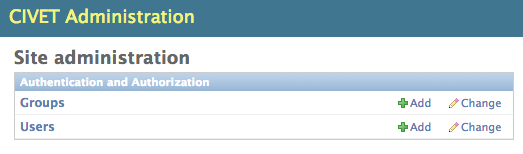
\includegraphics{adminpage.png}
\end{figure}

The \emph{Add} and \emph{Change} buttons provide access to a rich set of options for adding users and editing information about them.
Clicking on “Users” will give a screen listing all of the users in the system, and clicking on a user name on that screen
goes to a page with information about the user. You can delete one or more users from these screens; the “Groups” option
allows users to be organized into groups.


\section{Additional notes}
\label{authentication:additional-notes}\begin{enumerate}
\item {} 
Accessing the page without additional arguments automatically does a logout.

\end{enumerate}

2. Django provides an extensive set of utilities for resetting passwords: for the sake of simplicity. as well as removing a
possible venue for mischief, these have not been activated: it should be relatively simple to do this if you would like
to have that capability.
\begin{quote}

At the present time, the AWS deployment does not show the pretty form, but all of the options are still there and
function: this will be corrected at some future date.
\end{quote}
\begin{enumerate}
\setcounter{enumi}{2}
\item {} 
The GitHub version of the program is populated with at least the following:
\begin{quote}

Superuser: civet-super  Password: je-kiffe-grenouilles \footnote{
You were expecting “password”, “CHANGEME” or “12345678”??
}

User: ima-coder  Password: code-code-code!

For the sake of security, you will probably want to delete these after you create your own environment, or at
least change the passwords.
\end{quote}

\end{enumerate}


\chapter{Home Page Options}
\label{homepage:home-page-options}\label{homepage::doc}
The home page has the following links:
\begin{description}
\item[{\textbf{Read coding form:}}] \leavevmode
CIVET reads a coding form template without using a workspace: this
is used if you want to use the web coding form without annotated
texts. This option can also be used when debugging coding forms.

\item[{\textbf{Read workspace:}}] \leavevmode
CIVET reads a set of text collections and their associated coding
form from a zipped file: this mode allows for text annotation and
extraction and is described in more detail in Section
{[}sec:workspace{]}, {[}sec:annotate{]} and {[}sec:coding{]}.

\item[{\textbf{Manage workspace:}}] \leavevmode
This links to various utilities that operate on workspace files
including downloading the coded data as a
tab-delimited file, editing the meta-data, and adding comments to
the file. {[}Beta 0.9: only the data download is implemented; editing
the meta-data can be done in a text editor.{]}

\item[{\textbf{Set preferences:}}] \leavevmode
This goes to a page where various program preferences can be set
manually.

\end{description}

\textbf{Documentation}
\begin{quote}
\begin{description}
\item[{\textbf{On-line manual}}] \leavevmode
Links to an HTML version of the documentation

\item[{\textbf{Download PDF}}] \leavevmode
This downloads a PDF file with the documentation.

\end{description}
\end{quote}
\begin{description}
\item[{\textbf{Log out}}] \leavevmode
Log out the current user. You will only see this option if log-ins
are required: see the chapter on “Authentication.”

\end{description}


\section{File selection}
\label{homepage:file-selection}
The first three modes go to a file selection screen.
\begin{figure}[htbp]
\centering
\capstart

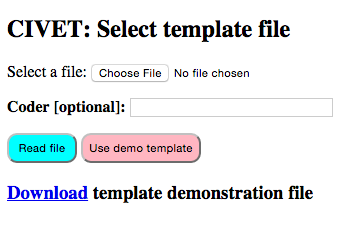
\includegraphics{fileselect.png}
\caption{CIVET file selection screen}\end{figure}

This provides the following options:
\begin{description}
\item[{Choose file:}] \leavevmode
Select a file containing a coding form template or workspace, then
read this into the system by clicking the \code{Read file} button.

\item[{Coder:}] \leavevmode
Any text entered here—typically a coder name or ID—will be included
as metadata with any annotations or cases coded. This field is
optional.

\item[{Demo file:}] \leavevmode
Read the simple demonstration files built into the system. \footnote{
These files are named \code{CIVET.demo.template.txt} and
\code{CIVET.extract.demo.zip} in the directory
\code{djcivet\_site/djciv\_data/static/djciv\_data/} and can be modified
there.
}

\item[{Download demonstration file:}] \leavevmode
This downloads a template or workspace demonstration file, which can
be used as an example.

\end{description}


\chapter{CIVET Coding Form Templates}
\label{forms:sec-forms}\label{forms:civet-coding-form-templates}\label{forms::doc}
A CIVET template file specifies the individual components of the form:
these are the familiar components from web forms but the syntax used to
specify them is simpler than what you will find in HTML.

CIVET is simply adding these controls to an HTML \code{\textless{}form\textgreater{}} and, as with
all things HTML, most of the placement of the fields is handled by the
browser. \footnote{
Writing in HTML5 and CSS, one can actually exercise a very fine
degree of control over the placement, but if you are comfortable with
that sort of code, you presumably aren’t using CIVET in the first
place. That said, you can see the HTML generated by CIVET by using
the \emph{View source} option in your browser, then save it as a file
using \emph{Save Page As...} and that could provide a starting point for
creating prettier code.
} CIVET provides some limited formatting through the
insertion of text and line breaks, and with some experimenting you
should be able to keep the form from being too ugly.

The template file should be a simple text file—most systems are happier
if this ends in the suffix \code{.txt}—similar to that used in an \emph{R}
or \emph{Stata} script (that is, not a formatted file such as that
produced by \emph{MS-Word}). Appendix 1 gives an example of a template
file, and the code for this can also be downloaded from a link in the
program.


\section{Simple Template-Based Data Entry Form}
\label{forms:simple-template-based-data-entry-form}
The basic data entry form just uses the presumably familiar standard
HTML data entry fields and should be self-explanatory.

To save a set of coded fields, click one of the buttons which follow the
title \code{Options after saving:}
\begin{description}
\item[{Code another case:}] \leavevmode
Save, then return to the same form

\item[{Download data:}] \leavevmode
Save, then download data as a tab-delimited text file

\end{description}

The \code{Download CIVET data} page  provides a
text box for a file name, and the \code{Download file} button downloads the
coded data. Use the \emph{Start new data file} link to re-start the coding
and the \emph{Continue coding with this file} link to continue adding to the
existing records.
\begin{itemize}
\item {} 
The .txt file is tab-delimited and contains the variable names in the
first line.

\item {} 
If the file name does not end in “.txt,” this suffix will be added.

\end{itemize}
\begin{figure}[htbp]
\centering

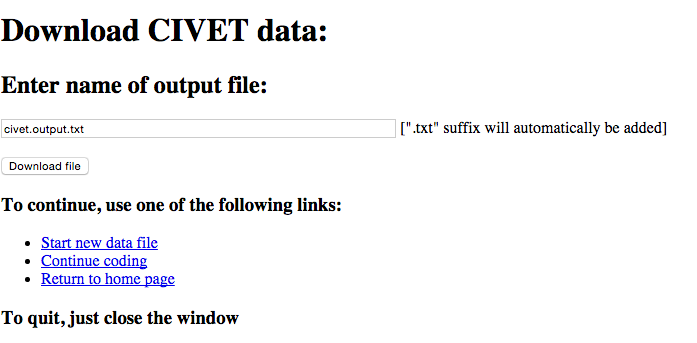
\includegraphics{download.png}
\end{figure}


\section{Command formats}
\label{forms:command-formats}
Commands generally have the following format

\begin{Verbatim}[commandchars=\\\{\}]
command: entry\PYGZhy{}title [var\PYGZhy{}name] options
comma\PYGZhy{}delimited list
\end{Verbatim}

Commands vary in how many of these components they have, but all follow
this general pattern.

Each command ends with a blank line (or, if you prefer, the commands are
separated by blank lines.)

Commands can also be cancelled by adding a “-” in front of the command:
this will cancel the entire command, that is, all of the lines
associated with the command, not just the first line. \footnote{
This feature is actually a bit more subtle: cancellation is invoked when
the first character in a line is “-” \emph{and} there is a “:” in the line,
which will always occur with a command. This allows default texts such as “- - -”
to be used, though a default text such as “- - -: we really want to confuse CIVET”
will cause an error.
}  For visual
symmetry, a “+” in front of the command “activates” it, though the
command will also be active without the plus.

“\#” denotes a comment: anything following a “\#” is ignored, so lines
beginning with “\#” are completely ignored.


\subsection{Items in template specification}
\label{forms:items-in-template-specification}
The commands involve one or more of the following items:
\begin{description}
\item[{entry-title}] \leavevmode
This is the title of data entry field. If this ends with \code{/} a
line-break (\code{\textless{}br\textgreater{}}) is inserted after the text. The titles are
escaped: at present the characters \textless{}, \textgreater{}and the single and double
quotes are replaced with the equivalent HTML entities
\code{\&lt;, \&gt; \&quot;} and \code{\&rsquo;}. \footnote{
In the current implementation, named HTML entities such as \code{\&copy;}
and \code{\&euro;} can be included and should produce the correct
character. At present numbered entities such as \code{\&\#91;}—the HTML
equivalent of ’{]}’—do not work since the \# is interpreted as a comment
delimiter: depending on whether there is demand for this feature, the
system could provide a way around this.
} The \textbf{entry-title}
field cannot contain the characters “{[}” or “{]}”—if these are present
they will be interpreted as bounding the \textbf{var-name} field—but the
escaped versions “\textbackslash{}{[}” and “\textbackslash{}{]}” are allowed.

\item[{var-name}] \leavevmode
The text of the variable name for this field; this will be used in
the first line of the \code{.csv} output file

\item[{comma-delimited-option-list}] \leavevmode
A list of the items that can be selected, separated by commas. A
‘*’ at the beginning of the item means that it will be initially
selected.

\item[{comma-delimited-var-name-list}] \leavevmode
A list of items which appear in \textbf{var-name} fields, separated by
commas.

\item[{page-text}] \leavevmode
Any text

\item[{number}] \leavevmode
An integer

\end{description}


\subsection{Errors in template commands}
\label{forms:errors-in-template-commands}
There is a fair amount of error trapping as the commands are processed;
any problems will reported on a web page. Generally the system will
stop after it has encountered the first error rather than reporting
all of the errors in the file.


\section{Specifying variables}
\label{forms:specifying-variables}

\subsection{Specifying variables to save}
\label{forms:specifying-variables-to-save}
This command gives the variables that will be saved; these can be in any
order but each of these must correspond to a \code{var-name} somewhere in
the form, or are one of the special variables discussed below. A
tab-delimited version of this list will be the first line of the output
file. The command can occur anywhere in the file.
\begin{quote}

\begin{DUlineblock}{0em}
\item[] \textbf{save:}
\item[] comma-delimited-var-name-list
\end{DUlineblock}
\end{quote}

If the variable name has brackets following it, the \emph{value} of the
variable rather than the literal text will be written when the data are
written to a tab-delimited file: the value is the string in brackets
\code{{[}…{]}} in the annotated coding mode. If there is a variable name inside
the brackets, that will be used as the column name for the values;
otherwise the regular name will be used: this allows both the literal
text and the value to be saved, as in the third example below.

If \code{save} specifies a value output and not is found, the output depends
on the preference \code{civet\_settings.USE\_TEXT\_FOR\_MISSING}, which also can
be set on the “Preferences” page. If this is \code{True}, the text will be
used; otherwise the string in  \code{civet\_settings.MISSING\_VALUE} will be used.

\textbf{Example:}

\begin{Verbatim}[commandchars=\\\{\}]
save:
worldregion, eyewit, groupname, comments

save:
worldregion [regioncode], eyewit, groupname[], comments

save:
worldregion, eyewit, groupname, groupname [groupcode], comments
\end{Verbatim}


\subsection{constant}
\label{forms:constant}
Sets the value of a variable to a constant; this can be used in a
\code{save:}
\begin{quote}

\begin{DUlineblock}{0em}
\item[] \textbf{constant:} page-text {[}varname{]}
\end{DUlineblock}
\end{quote}

\textbf{Example:}
\begin{quote}

\code{constant: Data set 0.2 {[}data\_id{]}}
\end{quote}


\subsection{filename}
\label{forms:filename}
Sets the default file name for the downloads: this can be changed before
downloading.
\begin{quote}

\begin{DUlineblock}{0em}
\item[] \textbf{filename:} page-text
\end{DUlineblock}
\end{quote}

\textbf{Example:}
\begin{quote}

\code{filename: our\_wonderful\_data.csv}
\end{quote}


\subsection{Special \texttt{save} variables}
\label{forms:special-save-variables}\begin{description}
\item[{\_coder\_}] \leavevmode
Coder text entered in the \emph{CIVET template selection} page

\item[{\_date\_}] \leavevmode
Current date. this is currently in the form YYYY-MM-DD. \footnote{
This format can be changed in the function \code{get\_special\_var(avar)} in
\emph{civet\_form.py}: It is specified using the extensive Python/C date format
operators shown \href{http://strftime.org/}{here.}
}

\item[{\_time\_}] \leavevmode
Current time in hh:mm:ss format

\end{description}


\section{Commands only relevant in workspaces}
\label{forms:commands-only-relevant-in-workspaces}

\subsection{discard}
\label{forms:discard}
Sets an initially unchecked checkbox for the special variable
“\_discard\_”, which can be used
to indicate that a collection has been evaluated by a coder but nothing
was coded. When this is checked, a case is generated for the collection
containing only the “\_discard\_” variable; those cases are not used to
generate data.
\begin{quote}

\begin{DUlineblock}{0em}
\item[] \textbf{discard:} entry-title
\end{DUlineblock}
\end{quote}

\textbf{Example:}
\begin{quote}

\code{discard: Texts are not codeable}
\end{quote}


\subsection{comments}
\label{forms:comments}
Creates a textarea box for the special variable \code{\_comments\_} which will be
added to the “casecmt” meta-data for the case being coded. \code{\_comments\_}
can also be added to the output data like any other variable, but this
is not required. The default size of the text box is 4 x 64 characters;
alternative sizes can be specified by adding an empty set of brackets
followed by \code{rows} and \code{cols} using the same format as the \code{textarea}
command. \footnote{
In fact, the \code{comments:} command is just a shorthand for
\code{textarea: entry-text {[}\_comments\_{]}}, and this will have the same
effect, with the contents added to the metadata.
}
\begin{quote}

\begin{DUlineblock}{0em}
\item[] \textbf{comments:} entry-title
\item[] \textbf{comments:} entry-title {[}{]} rows = number cols = number
\end{DUlineblock}
\end{quote}

\textbf{Example:}
\begin{quote}

\code{comments: Enter any additional comments about this case}
\end{quote}


\subsection{header}
\label{forms:header}
Sets the HTML code for the display of collection information at the
top of the editing and coding screens. The text of \code{field-name} will
be substituted for the optional token \code{\_text\_} in \code{HTML-text}
\begin{quote}

\begin{DUlineblock}{0em}
\item[] \textbf{header:} HTML-text {[}field-name{]}
\end{DUlineblock}
\end{quote}

\code{field name} should be one of the following
\begin{description}
\item[{\code{workspace}}] \leavevmode
Workspace file name

\item[{\code{collection}}] \leavevmode
Collection ID (\code{collid} field)

\item[{\code{comments}}] \leavevmode
Collection comments (\code{collcmt} field)

\end{description}

The three fields are displayed in this order; they default to null strings.
The individual \code{header} commands must be separated by blank lines; otherwise,
consistent with the command syntax, \footnote{
Neither a bug nor a feature: just is what it is.
} the latter lines will be ignored.

\textbf{Example:}

\begin{Verbatim}[commandchars=\\\{\}]
header: \PYGZlt{}h3\PYGZgt{}\PYGZlt{}span style=\PYGZdq{}color:blue\PYGZdq{}\PYGZgt{}Workspace \PYGZus{}text\PYGZus{} \PYGZlt{}/span\PYGZgt{}\PYGZlt{}/h3\PYGZgt{}\PYGZsq{} [workspace]

header: \PYGZlt{}b\PYGZgt{}Collection:\PYGZlt{}/b\PYGZgt{} \PYGZus{}text\PYGZus{} \PYGZsq{} [collection]
\end{Verbatim}


\subsection{Special \texttt{save} variables for workspaces}
\label{forms:special-save-variables-for-workspaces}
These variables will not include any texts that were deleted using
\code{shift-click} on the lede. \footnote{
At present, only these two fields are available, but it is relatively
straightforward to add the others by just following the existing
code that you locate in a search for “textpublisher”
}
\begin{description}
\item[{\_collection\_}] \leavevmode
\code{collid} field of the collection

\item[{\_publisher\_}] \leavevmode
Comma-delimited list of the \code{textpublisher} fields of the texts in
the collection

\item[{\_bibliorefs\_}] \leavevmode
Comma-delimited list of the \code{textbiblio} fields of the texts in
the collection

\end{description}


\section{Data entry fields}
\label{forms:data-entry-fields}
Any of these commands can be prefixed with “//”, which inserts a \code{\textless{}p\textgreater{}\textless{}/p\textgreater{}}
or a “/”, which inserts a \code{\textless{}br\textgreater{}}.


\subsection{\emph{checkbox}: Binary checkbox}
\label{forms:checkbox-binary-checkbox}
A simple binary check-box. The value of the variable will be first item
in the list when the box is not checked; the second item when the box is
checked. The * notation on the second item can be used to specify
whether or not the box is initially checked.
\begin{quote}

\begin{DUlineblock}{0em}
\item[] \textbf{select:} entry-title {[}var-name{]}
\item[] comma-delimited-option-list
\end{DUlineblock}
\end{quote}

\textbf{Example:}

\begin{Verbatim}[commandchars=\\\{\}]
checkbox: Eyewitness report? [eyewit]
no,*yes
\end{Verbatim}


\subsection{\emph{select}: Pull-down menu}
\label{forms:select-pull-down-menu}
Pull-down menus—which are called a “select” in HTML—are specified with
the syntax
\begin{quote}

\begin{DUlineblock}{0em}
\item[] \textbf{select:} entry-title {[}var-name{]}
\item[] comma-delimited-option-list
\end{DUlineblock}
\end{quote}

\textbf{Example:}

\begin{Verbatim}[commandchars=\\\{\}]
select: Region [worldregion]
North America, South America, Europe, *Africa, Middle East, Asia{}`{}`
\end{Verbatim}


\subsection{\emph{dynselect}: Select from dynamic pull-down menu {[}workspaces only{]}}
\label{forms:dynselect-select-from-dynamic-pull-down-menu-workspaces-only}
Pull-down menus which are specified dynamically using the \code{categories} section in the collections are specified with
the syntax
\begin{quote}

\begin{DUlineblock}{0em}
\item[] \textbf{dynselect:} entry-title {[}var-name{]}
\item[] category-name
\end{DUlineblock}
\end{quote}

\textbf{Example:}

\begin{Verbatim}[commandchars=\\\{\}]
select: Region [worldregion]
statelist
\end{Verbatim}

If the category-name is not found in the collection, the control defaults to a single entry \code{-{-}-}: this allows for
situations where there were no items found in the category.


\subsection{\emph{radio}: Radio buttons}
\label{forms:radio-radio-buttons}
A series of radio buttons are specified with the syntax
\begin{quote}

\begin{DUlineblock}{0em}
\item[] \textbf{radio:} entry-title {[}var-name{]}
\item[] comma-delimited-option-list
\end{DUlineblock}
\end{quote}

The entry \code{/} in the option list causes a line-break (\code{\textless{}br\textgreater{}}) to be
inserted

\textbf{Example:}

\begin{Verbatim}[commandchars=\\\{\}]
radio: Region [worldregion]
North America, South America, Europe, *Africa, /,Middle East, Asia
\end{Verbatim}


\subsection{\emph{textline}: Enter single line of text}
\label{forms:textline-enter-single-line-of-text}
This creates a box for a single line of text (HTML {}`{}` type=text{}`{}`). The
\code{width = number} is optional and specifies the size of the text entry
box in characters: the default is \code{width = 32}
\begin{quote}

\begin{DUlineblock}{0em}
\item[] \textbf{textline:} entry-title {[}var-name{]} width = number
\item[] initial-text
\end{DUlineblock}
\end{quote}

\textbf{Example:}

\begin{Verbatim}[commandchars=\\\{\}]
textline: Name of group [groupname]
\PYGZlt{}enter name\PYGZgt{}
\end{Verbatim}


\subsection{\emph{textclass}: Extract single line from annotated text}
\label{forms:textclass-extract-single-line-from-annotated-text}
This creates a box for a single line of text (HTML {}`{}` type=text{}`{}`) that
will interact with annotated text; in addition information can be
manually entered or cut-and-pasted into this box. If this command is
used in a form that does not have associated annotated text, it behaves
the same as \code{textline} and the \code{class} information is ignored.

The \code{class=class-name} is required and specifies the name of the
annotation class that the text-entry box is connected with; a class can
be associated with multiple text-entry boxes. There are four standard
classes:
\begin{itemize}
\item {} 
\code{nament}: named-enties, which are determined by capitalization

\item {} \begin{description}
\item[{\code{geogent}: geographical locations, which are determined by a}] \leavevmode
combination of prepositions and capitalization \footnote{
This is only done in the automatic annotation if
\code{civet\_settings.USE\_GEOG\_MARKUP = True}: see the discussion in the
\emph{Preferences} chapter.
}

\end{description}

\item {} 
\code{num}: numbers

\item {} 
\code{date}: dates

\end{itemize}

The \code{width = number} is optional and specifies the size of the text
entry box in characters: the default is \code{width = 32}
\begin{quote}

\begin{DUlineblock}{0em}
\item[] \textbf{textclass:} entry-title {[}var-name{]} class=class-name
width=number
\item[] initial-text
\end{DUlineblock}
\end{quote}

\textbf{Example:}

\begin{Verbatim}[commandchars=\\\{\}]
textclass: Name of city [cityname] class=nament
 \PYGZlt{}enter city\PYGZgt{}
\end{Verbatim}


\subsection{\emph{textarea}: Enter multiple lines of text}
\label{forms:textarea-enter-multiple-lines-of-text}
This corresponds to an HTML “TEXTAREA” object. The
\code{rows = number cols = number} is optional and specifies the size of
the text entry box in characters: the default is \code{rows = 4 cols = 80}
\begin{quote}

\begin{DUlineblock}{0em}
\item[] \textbf{textarea:} entry-title {[}var-name{]} rows = number cols = number
\item[] initial-text
\end{DUlineblock}
\end{quote}

\textbf{Example:}

\begin{Verbatim}[commandchars=\\\{\}]
textarea: Description [descript] rows = 2 cols = 64
Briefly describe the incident
\end{Verbatim}


\section{Linking fields}
\label{forms:linking-fields}

\subsection{\emph{link}: Linking \emph{select} and \emph{textline} fields}
\label{forms:link-linking-select-and-textline-fields}
The \textbf{link:} command can be used to connect a \textbf{select:} or \textbf{dynselect:} menu to a set of \textbf{textline:}
fields so that their content is filled in from the menu if something is selected, but otherwise these
fields can be filled in manually.
\begin{quote}

\begin{DUlineblock}{0em}
\item[] \textbf{link:} one-to-four-textline-vars {[}select-var-name{]}
\end{DUlineblock}
\end{quote}

The list of variables is space-delimited and all of the variables must have been defined before the \textbf{link:}
command is encountered, but otherwise the command can be anywhere in the file.

The rules for extracting the fields depends on the number of variables specified:
\begin{enumerate}
\item {} 
Insert the entire menu item, which can have any format, in the text field

\item {} 
The entire menu item has the form \code{xxxxx {[}yyy{]}}  The \code{xxxxx}—which can contain anything except
\code{{[} {]}}—is inserted in the first field; \code{yyy} is inserted in the second field. This is typically used for names
and codes, e.g. \code{Algeria {[}DZA{]}}

\item {} 
The entire menu item has the form \code{xxxxx (zzzz) {[}yyy{]}}  The \code{xxxxx}—which can contain anything except
\code{(  )}—is inserted in the first field; \code{zzzz} is inserted in the \emph{third} field, and \code{yyy} is inserted
in the second field. This a somewhat awkward generalization of the four-variable option.
Example: \code{Algiers (Algeria) {[}DZA{]}}

\item {} 
The entire menu item has the form \code{xxxxx (lat, lon) {[}yyy{]}}  The \code{xxxxx}—which can contain anything except
\code{(  )}—is inserted in the first field; \code{lat} is inserted  in the third field, \code{lon} in the fourth field,
and \code{yyy} is in the second field. This is typically used for names with geocoordinates and codes,
e.g. \code{Algiers (36.757, 3.063) {[}DZA{]}}, but \code{lat} and \code{lon} do not need to be numbers

\end{enumerate}

At present, there is only minimal error checking to insure that the fields are delimited correctly: These are taken
from a set menu, not user input, so it is the responsibility of the form developer to make sure these aren't ambiguous
(e.g. the menu option \code{Florence (Firenze) (43.821641, 11.286954) {[}ITA{]}} will generate the string \code{Firenze) (43.821641}
as the \emph{lon} field). Alternatively, you can add code in \code{civet\_coder.html} to accommodate the more complex formats.

\begin{Verbatim}[commandchars=\\\{\}]
link: countryname countrycode [countrymenu]

link: cname ccode clat clong [geolocmenu]
\end{Verbatim}


\subsection{\emph{textsource}: Extract sources from annotated text}
\label{forms:textsource-extract-sources-from-annotated-text}
A \code{textsource:} field can be automatically linked to a \code{textclass:}
field so that the information in the \code{textid:} and/or \code{textbiblio:} field
for the workspace text block where an annotated word or phrase has been
extracted will be automatically added. This linkage is done by using
the variable name from a \code{textclass} field with \code{\_src} added to the
end.

Except for the linkage, a \code{textsource} variable acts like a regular text
variable: information can be typed or pasted into the text box—typically this
will be done from the \code{Source} information that is visible when the
\code{Show Comments} option is active—and the variable can be saved.

If the variable name does not correspond to a \code{textclass} variable with
an added \code{\_src}, \code{textsource} behaves the same as \code{textline.}  \footnote{
In a future version of CIVET we hope to have a facility where citation
information can be transferred into a \code{textsource} field by clicking on
a lede but this has been implemented yet.
\emph{Preferences} chapter.
}

The \code{textid:/textbiblio:} content is controlled by the preferences
“Use textid in source citation:” and “Use textbiblio in source citation:”;
the default uses only \code{textbiblio:}.

The \code{width = number} is optional and specifies the size of the text
entry box in characters: the default is \code{width = 32}
\begin{quote}

\begin{DUlineblock}{0em}
\item[] \textbf{textsource:} entry-title {[}var-name{]}  width = number
\item[] initial-text
\end{DUlineblock}
\end{quote}

\textbf{Example:}

\begin{Verbatim}[commandchars=\\\{\}]
textsource: Source for city [cityname\PYGZus{}src] width=40
\PYGZlt{}enter source\PYGZgt{}
\end{Verbatim}


\section{Additional web page formatting}
\label{forms:additional-web-page-formatting}

\subsection{\emph{title}: Set page title}
\label{forms:title-set-page-title}
Sets the title of the web page: that is, the HTML{}`{}`\textless{}title\textgreater{}...\textless{}/title\textgreater{}{}`{}`
section of the header.
\begin{quote}

\begin{DUlineblock}{0em}
\item[] \textbf{title:} page-title
\end{DUlineblock}
\end{quote}

\textbf{Example:}
\begin{quote}

\code{title: CIVET-based coding form}
\end{quote}


\subsection{Insert text}
\label{forms:insert-text}
Adds text to the form: the various options follow the usual HTML
formats. In interests of simplicity, text is “escaped” so that special
characters are not interpreted as HTML: note that this means that
in-line mark-up such as \code{\textless{}i\textgreater{}}, \code{\textless{}b\textgreater{}} and \code{\textless{}tt\textgreater{}} will not work,
so if you need this activate and use the \code{html:} command. Also keep in
mind that these commands need to be separated by a blank line.

A “/” in the page-text will add a line-break \code{\textless{}br\textgreater{}}. To include a
“/” in the text, use “//”.
\begin{quote}

\begin{DUlineblock}{0em}
\item[] \textbf{h1:} page-text
\item[] \textbf{h2:} page-text
\item[] \textbf{h3:} page-text
\item[] \textbf{h4:} page-text
\item[] \textbf{p:} page-text
\end{DUlineblock}
\end{quote}

\textbf{Example:}

\begin{Verbatim}[commandchars=\\\{\}]
h1: Primary data set coding form

p:Please enter data in the fields below,/ and be really, really careful!
\end{Verbatim}

The simple command

\begin{Verbatim}[commandchars=\\\{\}]
p:
\end{Verbatim}

is useful for putting some space between form elements; this is equivalent to the
“//” prefix in the data entry commands.


\subsection{\emph{newline}: Insert a line break}
\label{forms:newline-insert-a-line-break}
Adds a new line in the form; this is equivalent to the “/” prefix in the
data entry commands.
\begin{quote}

\textbf{newline:}
\end{quote}


\subsection{\emph{newpage}: Insert a page break}
\label{forms:newpage-insert-a-page-break}
Adds a new page to the form.
\begin{quote}

\textbf{newpage:}
\end{quote}


\section{Advanced formating options}
\label{forms:advanced-formating-options}
A CIVET form is simply a web page, and consequently can be controlled by
the standard commands for displaying web pages, notably cascading style sheets (CSS).


\subsection{Set css}
\label{forms:set-css}
Adds the text which follows the command to the \code{\textless{}style\textgreater{}...\textless{}/style\textgreater{}} section
in the page head. The text block is terminated by a blank line.
\begin{quote}

\begin{DUlineblock}{0em}
\item[] \textbf{css:}
\item[] one or more lines of css definitions
\end{DUlineblock}
\end{quote}


\subsection{Set form division sizes}
\label{forms:set-form-division-sizes}
This is a short-cut that for most options just changes the size of various components in either of these
forms:
\begin{quote}

\begin{DUlineblock}{0em}
\item[] \textbf{size:} {[}division-name{]} width = \textless{}length\textgreater{} height = \textless{}length\textgreater{}
\item[] \textbf{size:} {[}division-name{]} width : \textless{}length\textgreater{}; height : \textless{}length\textgreater{}
\end{DUlineblock}
\end{quote}

\textless{}size\textgreater{} can be any of the CSS “length” formats: \href{http://www.w3schools.com/cssref/css\_units.asp}{http://www.w3schools.com/cssref/css\_units.asp}.

\emph{division-name} is one of the following:
\begin{description}
\item[{\emph{body}}] \leavevmode
over-all size of the page

\item[{\emph{civ-editor}}] \leavevmode
size of CKEditor text box on the annotation page

\item[{\emph{civ-text-display}}] \leavevmode
size of the scrolling text display on the coding page

\item[{\emph{civ-form}}] \leavevmode
size of the coding form created by the template in both the basic form and the coding page

\end{description}

\textbf{Notes:}
\begin{enumerate}
\item {} 
The system does not check for the validity of either the division names or the
CSS \emph{\textless{}length\textgreater{}} specification; if they can't be interpreted
they are ignored.

\item {} 
\code{size} commands can occur anywhere and can be combined with a \code{css} command:
if they occur before the \code{css} command the contents of \code{css} will override \code{size},
and vice-versa if they occur afterwards: the CSS string for the
\code{\textless{}style\textgreater{}...\textless{}/style\textgreater{}} section is assembled in the order the commands occur.

\item {} 
Because CSS doesn't use object-like inheritance, the \code{size: {[}body{]}}  command resets
\emph{all} of the properties of \code{body}, leaving only \code{width} and \code{height} set in the style, e.g.

\begin{Verbatim}[commandchars=\\\{\}]
body \PYGZob{}
    width:900px;
    height:700px;
\PYGZcb{}
\end{Verbatim}

If you want to change the size but also retain other characteristics, use \code{css}
to define the complete \code{body} style.

\item {} 
The \code{civ-editor} command changes the size in the configuration of CKEditor rather than
any CSS, so this name cannot be used in  \code{css:} (well, it can be used but it won't
do anything...). CKEditor does not allow the “\%” option to be used as a “height”:
see \href{http://docs.ckeditor.com/\#!/guide/dev\_size}{http://docs.ckeditor.com/\#!/guide/dev\_size}. The CKEditor defaults to the width
of the page (more or less) and a height of 200px.

\item {} 
The  \code{civ-form} and \code{civ-text-display} names correspond correspond to \code{\textless{}div class='name'\textgreater{}}
in the content of the form; you can modify these directly by using a \code{css:{}`{}`command.
The {}`{}`size} command resets the \emph{\textless{}name\textgreater{}-size} class, which only controls the size.

\end{enumerate}


\subsection{Insert HTML}
\label{forms:insert-html}
{[}This command may or may not be included in the operational version of
the system, as it provides some opportunities for mischief. Stay tuned.
It is in the code but currently deactivated; if you are installing your
own version of the system, it can be activated by setting
\code{civet\_settings.HTML\_OK = True}.{]}

Adds arbitrary HTML code without escaping.
\begin{quote}

\begin{DUlineblock}{0em}
\item[] \textbf{html:}
\item[] one or more lines of HTML
\end{DUlineblock}
\end{quote}


\chapter{CIVET Workspaces}
\label{workspaces:civet-workspaces}\label{workspaces::doc}
CIVET is part of a projected collection of open-source programs designed
to work with very large sets of small text files: in the domain of
contentious politics these are usually news articles but the issue of
managing very large databases of small texts extends well beyond this
application. For example, projects analyzing texts from legislative
debates, legislation, campaign web sites and blogs all have much the
same character when they are studied at a large scale.

In the CIVET system, files containing sets of individual stories are
called “collections”: these are typically multiple related news
stories—“texts”—from which one or more data records—“cases”—are coded.
These are stored in a YAML format \footnote{
\href{https://en.wikipedia.org/wiki/YAML}{https://en.wikipedia.org/wiki/YAML}
} which is a structured
human-readable text file containing a number of data fields; the details
of this are given in Appendix 2.

Sets of text collections are grouped into “workspaces” that also contain
an associated coding form and, optionally, other information such as
user-specified categories that will be used in automatic annotation. The
template file begins with the string “\code{form.}” and uses the category
and template commands described in the chapter \emph{CIVET Coding Form Templates}.
Workspaces are compressed (\code{.zip}) directories (folders).

In the current configuration of the system, workspace files are uploaded
to the system, annotated and/or coded, then downloaded when a session is
completed: no data remain on the machine where the CIVET system is
running. In a future version, we expect to have an option for persistent
data that could be used on a secure server, as well as options for
reading these files from a server.

The workspace will generally \emph{not} be downloaded to the same place it
was originally: as a standard HTML security feature, the system does not
retain any information about where it obtained a file. Instead, it will
be downloaded to wherever your system downloads file: for example on the
Macintosh this is a folder named \code{Downloads}. \footnote{
If you read the workspace from the same directory where it will
eventually be downloaded, the behavior presumably depends on the
operating system: in the case of OS-X both the downloaded
file and the decompressed versions get a suffix added. E.g. if the
original workspace folder is named “test123” with the compressed
version “test123.zip”, the system assigns the downloaded version
the name “test123 (1).zip” which decompressed to a folder named
“test123 (1)”. We are leaving the task of insuring that the
original file is not over-written to the operating system and
whatever other utilities you might be using to manage workspaces.
} If you wish to
replace the original workspace file, this will need to be done manually
or with a script operating locally.

There is some limited error checking as the workspace is processed. If
errors are found you will get a screen similar to the figure
below listing the errors, which must be corrected before the
workspace can be used.
\begin{figure}[htbp]
\centering

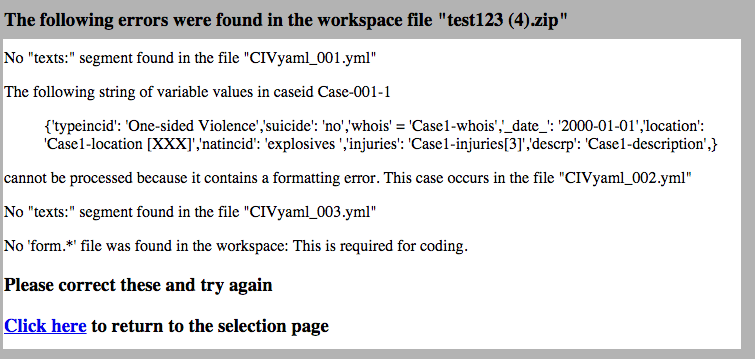
\includegraphics{workspace_errors.png}
\end{figure}

Like error messages in all programs, these are self-explanatory \footnote{
Hahaha…just a little programmer joke…
}
though in general errors will occur either when you are processing a
workspace for the first time or if you have manually edited it outside
of the CIVET system: once a workspace has been successfully read by
CIVET the program should not introduce any errors that would be caught
at this point. \footnote{
For example, the error in the variable values string in the example screen
occurs because of the substring
\code{'whois'='Case1-whois',} which should actually be
\code{'whois':'Case1-whois',} but that ‘\code{=}’ could only have been
introduced through external editing.
}

The program is sensitive to file names:
\begin{itemize}
\item {} 
Any file ending with \code{.yml} is assumed to be a CIVET -formatted
collections file

\item {} 
There should be one and only file beginning with the string
\code{form.}: this specifies the coding form for the workspace

\item {} 
Any file beginning with \code{codes.} is assumed to be a
{\hyperref[workspaces:sec-categories]{\emph{\DUspan{}{category vocabulary list}}}}. In the file name,
``codes.'' must be followed by a
\code{category} name then a period; the remainder of a ``codes'' file
name can be anything, though typically it will end in \code{.txt}.

\item {} 
Any file ending with \code{.ini} is assumed to be a configuration file
{[}Version 1.0: Not yet implemented—see comments on setting globals in
the “Preferences” chapter.{]}

\end{itemize}

Except for these restrictions, the directory can contain additional
files of any kind: these will be preserved when the file is downloaded.
A workspace file cannot contain subdirectories.

Additional notes on workspaces:
\begin{itemize}
\item {} 
So long as the YAML formatting is preserved—which should be fairly
straightforward—the system is indifferent as to whether editing is
done inside or outside of CIVET .

\item {} 
If the \code{form} file is missing or contains errors, the system will
display the errors it found, then return to the data selection page.

\item {} 
If you are manually editing the variable values in the \code{cases}
section, any single quotes (\code{’}) must be “escaped”; that is,
replaced with \code{\textbackslash{}’}. This will be done automatically when cases are
generated from inside the program.

\item {} 
The system currently translates UTF-8 encodings to ASCII \footnote{
\href{https://en.wikipedia.org/wiki/UTF-8}{UTF-8} is an expanded
\href{https://en.wikipedia.org/wiki/Unicode}{UniCode} character set that includes
accented letters, “smart quotes”
and many many more characters not found in the older
\href{https://en.wikipedia.org/wiki/ASCII}{ASCII} (American Standard Code for
Information Interchange) character set. UTF-8 is very widely used on the
Web so if you have downloaded texts, there's a pretty good change they
contain at least some UTF-8 characters.
} using the
Django function \code{encoding.smart\_str()}. We expect to eventually
convert the program to Python 3.x (at present it is Python 2.7) which
is utf-8 “native” but it isn't there yet.

\end{itemize}


\section{Workspace Management}
\label{workspaces:workspace-management}\label{workspaces:sec-management}
The \code{Manage workspace} link on the home page will take you first to a
workspace selection page, and then to the page shown below. In Beta 0.9, only the
\code{Export data in tab-delimited format/Use save-variable list in the template}
is implemented: this will download any coded cases found in the
workspace. The remaining functions will eventually be implemented but in
the meantime these tasks can be done using a text editing program.
\begin{figure}[htbp]
\centering

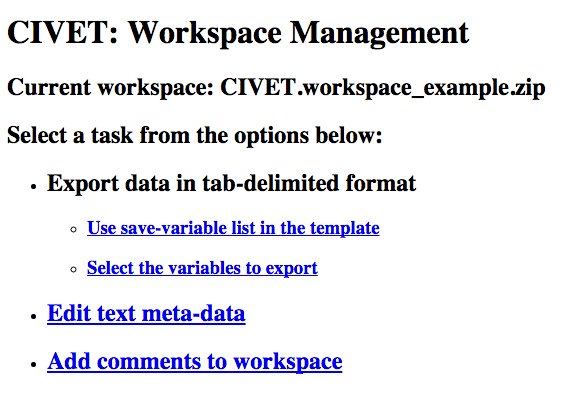
\includegraphics{manage.png}
\end{figure}


\section{User-specified annotation vocabulary using \textbf{category}}
\label{workspaces:sec-categories}\label{workspaces:user-specified-annotation-vocabulary-using-category}
The \code{category} command is used to set up special categories of words
that will be color-coded and can be associated with text-extraction
fields. The annotation can either be done automatically or by manually
selecting the text and using the \code{Style} pull-down menu in the
annotation editor.
\begin{quote}

\begin{DUlineblock}{0em}
\item[] \textbf{category:} category-name {[}color{]}
\item[] comma-delimited-phrase/code-list or file-name
\end{DUlineblock}
\end{quote}

The \code{category-name} must be unique and cannot be one of the standard
categories \code{nament, num} or \code{date}. The program currently
accommodates up to 99 categories. \footnote{
If you need more, this can be changed by allowing more digits in
the \code{\{:02d\}} format in the code
\code{UserCategories{[}newcat{]}.append('termst\{:02d\}'.format(len(UserCategories)))}
in \code{CIVET\_template.make\_category()}
}

\begin{DUlineblock}{0em}
\item[] \code{color} can be any of the 140 named HTML5 colors, \footnote{
See \href{http://www.w3schools.com/html/html}{http://www.w3schools.com/html/html} colornames.asp
} a six-digit
hexadecimal RGB color (e.g. \code{6A5ACD} corresponds to the named color
“SlateBlue”; the hex notation provides a presumably sufficient choice
of 16,777,216 colors), or a two-digit color from the CIVET
palette. \footnote{
This palette was assembled in a very ad hoc manner, is not
color-blind-friendly, and we would be delighted to substitute
something better. The list is set as \code{CIV\_template.CatColorList}
} The palette, shown below, can be
accessed by entering the address
\end{DUlineblock}
\begin{quote}

\href{http://127.0.0.1:8000/djciv\_data/make\_color\_list}{http://127.0.0.1:8000/djciv\_data/make\_color\_list}
\end{quote}

\begin{DUlineblock}{0em}
\item[] while the program is running on a dedicated machine. If \code{{[}color{]}} is
empty—that is, \code{{[}{]}}—the system uses a color from the standard list
in the listed order.
\end{DUlineblock}
\begin{figure}[htbp]
\centering

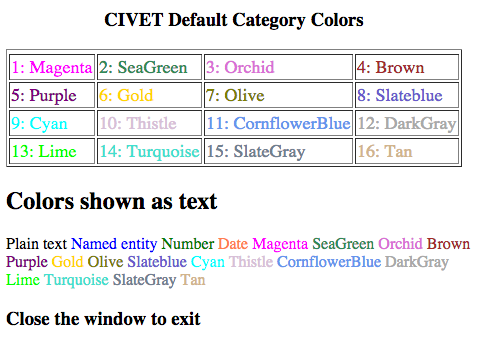
\includegraphics{defaultcolors.png}
\end{figure}


\section{Automatic annotation/skip editing mode only:}
\label{workspaces:automatic-annotation-skip-editing-mode-only}
When the program is running with \code{Always apply annotation: True} and
\code{Skip editing: True}, \footnote{
This is the configuration typically used when just coding the texts
with automated annotation. We plan to retrofit this to the editor
as well but adding it to the annotation was a simple hack, and adding
it to the editor is a little more complicated.
} categories can be further visually differentiated using
one or more of the following font specifications
\begin{itemize}
\item {} 
bold: \textbf{bold face}

\item {} 
italic: \emph{italic}

\item {} 
under: underline

\end{itemize}

So for example \code{{[}Green bold italic{]}} will display the category in an
italic bold font colored green.


\section{Additional information on categories}
\label{workspaces:additional-information-on-categories}
1. Generally, matching of words and phrases is not case sensitive: in
the example below, both ``killed'' and ``Killed'' will match. However, if the
word in the category list is all uppercase—e.g. NATO, IRA, ISIS—it will
only match all-uppercase strings: this should deal with most cases of
acronyms, in particular US and IS. A word or
phrase can only be in a a single category: putting one in multiple
categories will not cause an error, but only the first category
evaluated—generally this will occur in the order the categories were
entered—will be marked. Words and phrases within a category are
evaluated in the order they are listed—see the example in the chapter on annotation—
which can be used to establish precedent when words or
phrases overlap. At present the program does not allow partial matches,
though a facility for this may be added in the future. \footnote{
If you want it now, delete the test \code{if endx == idx+len(st):} in
\code{CIVET\_utilities.do\_string\_markup()}.
}

2. The comma-delimited-phrase/code-list can have codes assigned to each of
the phrases: these occur in brackets following the phrase and are added
to the text during automated markup. The codes can be any character
string. Either the phrase or the code or both can be specified in the
output. If some of the phrases in the list have codes and others do not,
the blank codes will be assigned a null (or, optionally, missing)
string.

3. The vocabulary list can also be read from a file in the workspace. The
file name must begin with \code{codes.category-name.}; the remainder of
the file name can be anything. \footnote{
The period following the category-name is required!: the file name
\code{codes.weapons\_mnsa\_list.txt} would not be recognized as a valid
\code{codes.} file. Or rather it would be interpreted as applying to a
category \code{weapons\_mnsa\_list}, not the category \code{weapons}.
} This be a text file with one phrase
per line and the code in brackets; a line beginning with \# is treated as
a comment.
\begin{enumerate}
\setcounter{enumi}{3}
\item {} 
As with texts, UTF-8 encodings are translated to ASCII using the
Django function \code{encoding.smart\_str()}.

\end{enumerate}

\textbf{Example:}

\begin{Verbatim}[commandchars=\\\{\}]
category:action [red italic]
killed [1], wounded [2], shot and killed [1], bombed [3], clashed [3]

category:people [Brown]
civilians, workers, authorities, troops, soldiers, rebels, people, group{}`{}`

category:nationstate [Gold bold under]
codes.nationstate.txt

category:weapons [Olive]
codes.weapons.mnsa.weaponslist\PYGZus{}150724.txt
\end{Verbatim}


\chapter{Annotation and Editing Collections}
\label{annotation::doc}\label{annotation:annotation-and-editing-collections}
The annotation and editing page for workspace collections \footnote{
If you are not seeing this screen,  \code{civet\_settings.SKIP\_EDITING} is
probably set to \code{True}: this can be changed on the “Preferences”
screen.
} implements a
minimal version \footnote{
that is, the version of \code{ckeditor} deliberately uses only a very
small set of the features that are available for the editor: if you
want to customize this, additional features can easily be added.
} of the open source Javascript “CKEditor” \href{http://ckeditor.com/}{http://ckeditor.com/} which allows the
texts to be edited and annotated. Editing works as you would expect,
including cut/copy/paste options.

Annotation is handled with the \code{Styles} drop-down menu in the window
toolbar which should show both
the standard CIVET categories—named-entity, number and date— and any
user-specified categories. To annotate, just select the text you want to
annotate and then select the annotation to apply.
\begin{figure}[htbp]
\centering

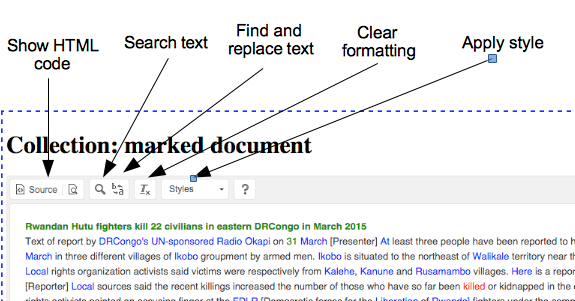
\includegraphics{ckedit_menu.png}
\end{figure}
\begin{figure}[htbp]
\centering

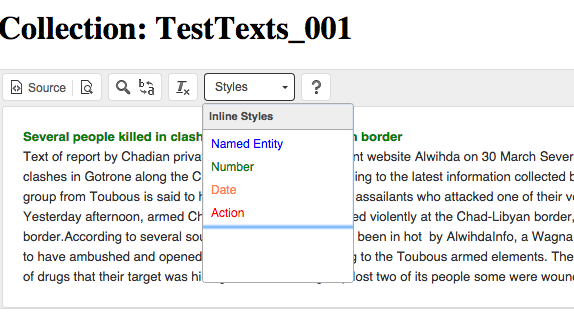
\includegraphics{style_options.png}
\end{figure}

The following options are available on this screen

\textbf{Annotate the collection:}
\begin{quote}

This applies the automated markup system which currently annotates the following
categories of words and phrases:
\begin{description}
\item[{\emph{Named-entities}:}] \leavevmode
This is based on capitalization; consecutive capitalized words
are combined.

\item[{\emph{Location} {[}optional{]}}] \leavevmode
When the \code{Use preposition-based geographical markup} preference is set to
\code{True}, these are named-entities which are preceded somewhere in the
text by prepositions in the list \code{'at','to','in','from'} See
additional discussion in the “Preferences” chapter.

\item[{\emph{Numbers}:}] \leavevmode
Digits and numerical words and phrases such as “one” and
“two-hundred.”

\item[{\emph{User-specified categories}:}] \leavevmode
See the discussion of {\hyperref[workspaces:sec-categories]{\emph{\DUspan{}{categories}}}}

\end{description}

Annotation is done automatically when \code{Always apply annotation} preference is
set to \code{True}; this can be changed on the “Preferences” screen.
\end{quote}

\textbf{Save edits and select new collection:}
\begin{quote}

This saves whatever annotation has been done to the internal
database \footnote{
That is, the data is saved on the machine where CIVET is running; it
is not saved on your local machine until the workspace is downloaded.
} and returns to the collection selection screen :
this option would be used if you are only annotating text rather
than coding them. Annotations are saved in the \code{textmkup} field
of the YAML file along with the date of the annotating and the
coder ID.
\end{quote}

\textbf{Save edits and code the collection:}
\begin{quote}

This saves whatever annotation has been done to the internal
database and goes to the coding and text extraction page
\end{quote}

\textbf{Discard edits and select new collection:}
\begin{quote}

This discards the edits and returns to the collection selection screen.
\end{quote}

\textbf{Download workspace and return to home screen:}
\begin{quote}

This downloads the current workspace without doing any coding.
\end{quote}


\section{Comments on annotation and editing}
\label{annotation:comments-on-annotation-and-editing}\begin{enumerate}
\item {} 
Associated codes in brackets following a term can be edited: when
writing variable values, the system will simply be looking for a
value in a bracket that occurs at the end of a string.

\item {} 
A word or phrase can be annotated only once. \footnote{
It would be possible to modify the system to allow for phrases to be
in multiple categories, but at present this seems like a low
priority; such a feature may or may not be included in future
versions.
} The user-specified
\code{category} words are annotated before the general named-entity, so
if a named entity occurs in a \code{category}, that will take
precedence. Similarly, any numbers that occur in a \code{category}
phrase will be part of the phrase, not separately marked as numbers.

\item {} 
Words and phrases in \code{category} lists are evaluated in the order
they are listed, which can be used to establish precedence.

Consider the sentence

\end{enumerate}
\begin{figure}[htbp]
\centering
\capstart


\includegraphics{annotation0.png}
\caption{The category listing:}{\small 
\begin{Verbatim}[commandchars=\\\{\}]
category:action [red]
shot and killed [4], killed [1], wounded [2], bombed [3]
\end{Verbatim}

would result in the annotation
}\end{figure}
\begin{figure}[htbp]
\centering
\capstart


\includegraphics{annotation1.png}
\caption{whereas category listing:}{\small 
\begin{Verbatim}[commandchars=\\\{\}]
category:action [red]
killed [1], shot and killed [4], wounded [2], bombed [3]]
\end{Verbatim}

would result in the annotation
}\end{figure}
\begin{figure}[htbp]
\centering
\capstart


\includegraphics{annotation2.png}
\caption{because the “killed” part of the phrase “shot and killed” has
already been annotated, and the remainder does not fit any of the
patterns.}\end{figure}
\begin{enumerate}
\setcounter{enumi}{3}
\item {} 
CIVET does not identify a capitalized word as a named-entity if it occurs as a single
word and is in the list of common “stop words” in the file
\begin{quote}

\code{djcivet\_site/djciv\_data/static/djciv\_data/CIVET.stopwords.txt}
\end{quote}

In other words, “The” will be included as part of a named-entity in the phrase
“The New York Times” but not in the phrase “The village was…”

\item {} 
Words referring to numbers such as “one”, “ten” and “fifty” have the corresponding
numerical value added in brackets following the number; these phrase and their
associated values are obtained from the file

\code{djcivet\_site/djciv\_data/static/djciv\_data/CIVET.numberwords.txt} \footnote{
Looking for a little programming exercise?: This needs more
development in at least three ways. First, generate all of the
standard English equivalents, e.g. “eighty-five”, since these follow
a simple set of rules. Second, and perhaps more important, allow the
user to specify the values for common approximations such as
“several,”, “many” and “dozens.” The second can be done by just
editing the file \code{CIVET.numberwords.txt}, though generally we don’t
want the user to have to figure out how to do that. Finally, there
should probably be some error checking to make sure the value in
brackets is actually a number: CIVET will just copy the value in
brackets without trying to convert it, but non-numbers will
presumably create issues further down the processing pipeline.
}

This file only contains the most commonly-encountered phrases; bracketed values can be added manually as well.

\end{enumerate}
\begin{enumerate}
\setcounter{enumi}{4}
\item {} 
At present, CIVET does not recognize leading punctuation—typically
quotes—and will not automatically mark named entities or numbers
beginning with this: this is on the list of changes for the future.
It does handle most trailing punctuation. In named entities, the
lower-case prefixes “al-”, “bin-” and “ibn-” are recognized as
part of a name. \footnote{
This list can be extended in the regular expression \code{pat1} in
\code{civet\_utilities.do\_NE\_markup()}.
}

\end{enumerate}


\chapter{Coding and Text Extraction}
\label{extraction::doc}\label{extraction:coding-and-text-extraction}
The CIVET coding form screen in the demonstration version is shown below. \footnote{
The form displayed is specified in the file

\code{djcivet\_site/djciv\_data/static/djciv\_data/CIVET.demo.coder.template.txt}

and can be modified if you want to experiment.
}
\begin{figure}[htbp]
\centering

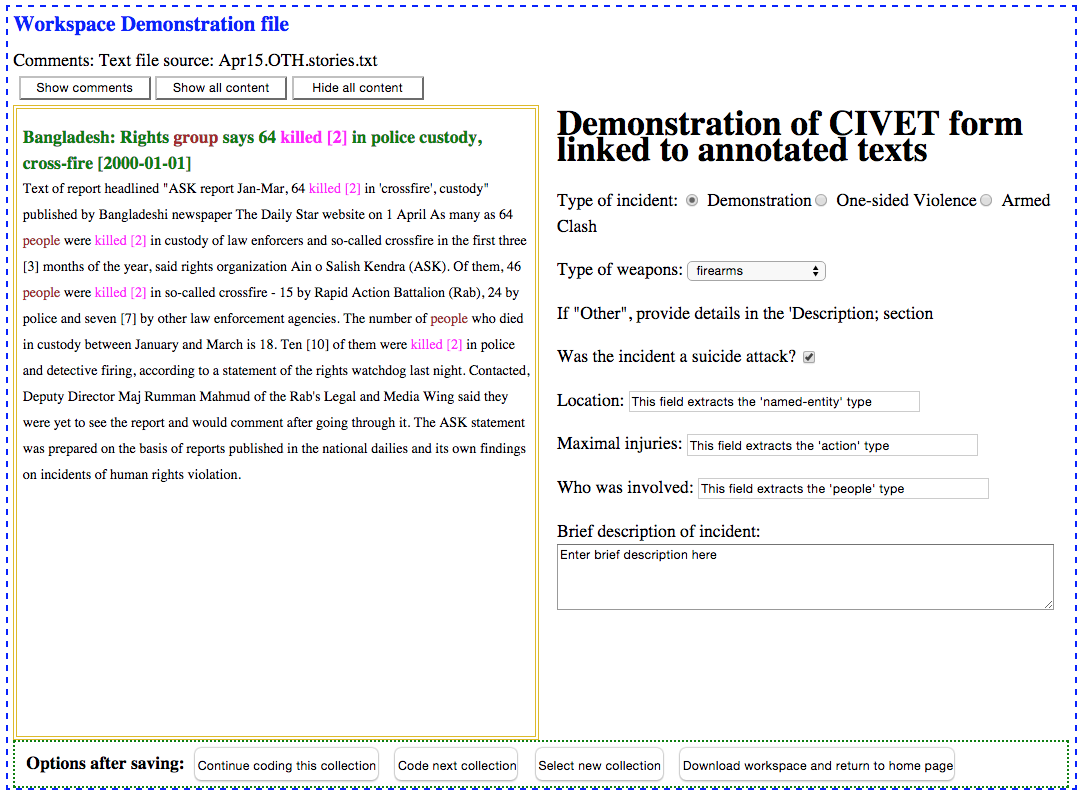
\includegraphics[width=0.800\linewidth]{civetcoder.png}
\end{figure}

The general operation of the coder/extractor is described below:
\begin{enumerate}
\item {} 
Unless \code{civet\_settings.SHOW\_ALL\_CONTENT = True}, only the content
of the first text will be expanded; to expand or collapse these,
click on the lede (green text). \footnote{
If you are switching back to the text from a text-extraction box,
you will need to double-click: the first click switches the focus
to the text; the second toggles the content
} The date of the
article follows the lede in brackets.

Shift-click on the lede will \emph{delete} the text: the lede and text
disappear and from any subsequent codings. The text actually remains
in the workspace file until it is permanently removed (or the
deletion is reversed) in the workspace management. See the notes
below for more details on this operation.

\item {} 
There are three controls at the top of the text display:
\begin{itemize}
\item {} \begin{description}
\item[{\code{Show/hide comments}: toggles the display of the comments and}] \leavevmode
sources for each text: these are initially hidden.  \footnote{
If the \code{textcmt} field for the text block was empty, the display will show
\code{Comment: -{-}-{-}}. If the \code{textbiblio} field for the text block was empty,
no \code{Source:} line will be shown.
}

\end{description}

\item {} 
\code{Show all content}: shows the content for all of the ledes

\item {} 
\code{Hide all content}: hides the content for all of the ledes

\end{itemize}

\item {} 
Clicking a text entry boxes associated with an annotation category
will highlight the relevant words in text: In the demonstration
version these are
\begin{description}
\item[{Location:}] \leavevmode
named-entities

\item[{Maximal injuries:}] \leavevmode
actions

\item[{Who was involved:}] \leavevmode
people

\end{description}

The ‘tab’ key cycles between the coding fields, or an option can be
selected using the mouse.

\item {} 
When an annotated category field is active, all of the words and
phrases in the text for that category are changed to red, with the
first word that is in an expanded text highlighted using a green
background. The arrow keys can
be used to move the highlighted text into the field. These operate as
follows:
\begin{description}
\item[{Right arrow:}] \leavevmode
Highlight the next text in the category

\item[{Left arrow:}] \leavevmode
Highlight the previous text in the category

\item[{Down arrow:}] \leavevmode
\emph{Replace} the contents of the field with the highlighted
text.

\item[{Up arrow:}] \leavevmode
\emph{Append} the contents of the field with the highlighted text.
The appended texts are comma-delimited.

\end{description}

If the highlighted text is off the screen, the window will automatically
scroll to place the text on the bottom of the screen. If the text
contains no words in the category, a pop-up window will alert you
to this.

If an annotated category field has an associated source field, that
information will be automatically replaced or added when the down
or up arrow is used. If a reference is already in the source field
and information is being added from the same source, this will not
be repeated. References can also be added to source fields using
copy-and-paste.

\textbf{Note:} If there are a number of phrases in the target category—this occurs
frequently for the named-entity and geographical-entity categories—and
the phrase you want to extract is not in the first
expanded block, click on the ledes to collapse them until you get
to a text that does contain the target phrase. If the earlier ledes
collapsed, the first phrase highlighted will be in the expanded
lede, so you will not need to hit the right-arrow key many times
to highlight and extract it.

\item {} 
Copy-and-paste from the text to the data fields work as you would
expect; text can also be entered and edited manually.

\item {} 
If bracketed values are included in the string, the system takes
the value from within a set of brackets that is the final item \footnote{
Specifically, the system checks whether the final character in the
string that is not whitespace is ‘{]}’. The output when the system is
expecting to find a bracketed value and does not is controlled by
the preference \code{civet\_settings.USE\_TEXT\_FOR\_MISSING} which can be
changed on the “Preferences” screen.
}
in the phrase: earlier sets are
assumed to be part of the text. For example, the value of the
phrase \code{Islamic State {[}ISIS{]}{[}mnsa{]}} will be “mnsa”; the value
of the phrase \code{Islamic State {[}ISIS{]} militia} will be
“Islamic State {[}ISIS{]} militia”.

\item {} 
To save a set of coded fields, click one of the buttons along the
bottom. At present, all three buttons save; later versions add
``cancel“ and ``reset” options. The options are:
\begin{description}
\item[{Continue coding this collection:}] \leavevmode
Save the data internally, then return to the same text to code
additional cases.

\item[{Code next collection:}] \leavevmode
Save the data internally, then select the next collection in the
workspace and go to the annotation screen.

\item[{Select new collection:}] \leavevmode
Save the data internally, then select a new collection

\item[{Download workspace and return to home screen:}] \leavevmode
This downloads the workspace with the coded cases to the local
machine. The {\hyperref[workspaces:sec-management]{\emph{\DUspan{}{Manage workspace}}}} facility  can then be used to download any coded cases.

\end{description}

\end{enumerate}


\section{Note on deleting texts}
\label{extraction:note-on-deleting-texts}
Deleting a text changes the value of the \code{textdelete} field to
\code{True}: the text remains in the workspace file but will not be
displayed again. Deletion also generates a case with the standard
\code{casedate} and \code{casecoder} fields and the following fields in the
\code{casevalues} dictionary

\begin{Verbatim}[commandchars=\\\{\}]
\PYGZus{}delete\PYGZus{} : True
\PYGZus{}textid\PYGZus{} : textid for the deleted text
\end{Verbatim}

This can be used to track the deletion of specific texts. version
Beta-0.9 does not have any internal utilities for using this
information but those functions may be added in a later version.

Deletion is tracked through the hidden text field \code{deletelist}
in \emph{civet\_coder.html.}


\chapter{Preferences}
\label{preferences::doc}\label{preferences:preferences}
This page has standard HTML check-boxes for setting the status of some of the
variables affecting the work flow and initial presentation of the texts.

\textbf{Note:} The “Default” values are those in the “off-the-shelf” version of the
program: if you are using a version that has been customized for your specific
project, these may have been changed. And if so, further changing them may have
unpredictable consequences for the proper functioning of the program.
\begin{description}
\item[{\textbf{Always apply annotation}}] \leavevmode
Always apply automatic annotation to texts that have not been previously
annotated.
\begin{itemize}
\item {} 
Default: \code{True}

\item {} 
“civet\_settings.py” variable: \code{ALWAYS\_ANNOTATE}

\end{itemize}

\item[{\textbf{Never apply annotation}}] \leavevmode
Never apply automatic annotation to texts: this is used when the annotation has
already been done in the YAML file. When \code{True},  the
“Code next collection” button in the coding screen will read the next
collection then display the text with the form without any additional
markup.
\begin{itemize}
\item {} 
Default: \code{False}

\item {} 
“civet\_settings.py” variable: \code{NEVER\_ANNOTATE}

\end{itemize}

\item[{\textbf{Show all content in coder}}] \leavevmode
In the coder, initially expand the content of all of the ledes.
\begin{itemize}
\item {} 
Default: Only expand the first lede.

\item {} 
“civet\_settings.py” variable: \code{SHOW\_ALL\_CONTENT}

\end{itemize}

\item[{\textbf{Skip editing}}] \leavevmode
When reading a collection, skip the editing screen and go directly to the
coder: this is typically used when dealing with texts that have already
been annotated or where the form does not have any fields that use
annotation.

When combined with \code{Always apply annotation: True}, the
“Code next collection” button in the coding screen will read the next
collection, apply the automatic annotation, and display the annotated
text with the form. In this mode, the automatic annotation is not
saved.
\begin{itemize}
\item {} 
Default: \code{False}

\item {} 
“civet\_settings.py” variable: \code{SKIP\_EDITING}

\end{itemize}

\item[{\textbf{Use text if value is missing:}}] \leavevmode
This controls the output when \code{save} specifies a value output and a
bracketed value is not the final element of the text string.  If \code{True},
the text will be
used; otherwise the MISSING\_VALUE string will be used.

When combined with \code{Always apply annotation: True}, the
“Code next collection” button in the coding screen will read the next
collection, apply the automatic annotation, and display the annotated
text with the form. In this mode, the automatic annotation is not
saved.
\begin{itemize}
\item {} 
Default: \code{True}

\item {} 
“civet\_settings.py” variable: \code{USE\_TEXT\_FOR\_MISSING}

\end{itemize}

\item[{\textbf{Use preposition-based geographical markup:}}] \leavevmode
Use prepositions to attempt to identify named entities that are geographical
locations: capitalized phrases that are preceded by the prepositions in the
list \code{'at','to','in','from'} are assigned the category “Location”. If a
phrase is identified \emph{anywhere} in the text as a possible
locations, all instances will be labelled with that category; that
label will take precedence over the standard “Named entity” category.
\begin{itemize}
\item {} 
Default: \code{False}

\item {} 
“civet\_settings.py” variable: \code{USE\_GEOG\_MARKUP}

\item {} 
“civet\_settings.py” preposition list: \code{GEOG\_PREPOSITIONS}

\end{itemize}

\end{description}

\textbf{Use textid in source citation:}
\begin{description}
\item[{\textbf{Use textbiblio in source citation:}}] \leavevmode
These control the content of the \code{Source:} that is saved in a \code{textsource}
command and displayed in the \code{Comments:} \code{textid} and \code{textbiblio}
refer to the fields in the texts in a workspace file. When both are true,
the source has the form “textid:textbiblio” where the content of the
field is substituted for the name, unless \code{textbiblio} is empty, in which
case it has the form “textid”. If only one is true, only
the contents of that field are included; if both are false, the source is
empty and not shown.
\begin{itemize}
\item {} \begin{description}
\item[{Default:}] \leavevmode
textid: \code{False}

textbiblio: \code{True}

\end{description}

\item {} 
“civet\_settings.py” variables: \code{USE\_TEXTID\_IN\_SOURCE}, \code{USE\_TEXTBIBLIO\_IN\_SOURCE}

\end{itemize}

\item[{\textbf{Missing value}}] \leavevmode
Sets the missing value.
\begin{itemize}
\item {} 
Default: *

\item {} 
“civet\_settings.py” variable: \code{MISSING\_VALUE}

\end{itemize}

\end{description}


\section{Programming note}
\label{preferences:programming-note}
We eventually expect to implement an option for setting initial preferences
through a configuration file in the workspace, but in the meantime the default
values of various global variables are set in the file
\emph{civet\_settings.py} and should be reasonably well documented there; in most
cases these take the values \code{True} or \code{False}; those values are
case-sensitive.

The preferences page is implemented through those global variables, a very
minimal Django form class \code{PrefsForm} in \emph{forms.py}, and the \code{set\_preferences()}
and \code{get\_preferences()} functions in \emph{civet\_settings.py.}  If you wish
to make additional global variables modifiable from this screen,  you will probably be able to
customize it just by following the examples in the existing code.


\chapter{Projected Features}
\label{future::doc}\label{future:projected-features}
CIVET is part of a projected system designed for managing
tens-of-thousands, or even millions, of small text files. The transition
in the past three decades from paper-based to electronic sources has
dramatically increased the amount of information that can potentially be
coded, but results in a “drinking from a fire hose” problem where a huge
number of false positives must be managed because typically only a very
small percentage of the texts obtained for a project actually contain
unique codeable events: yields of 1\% to 3\% are not uncommon. There is
very little existing software designed to deal with this situation,
since the texts are too large to be treated as nominal variables in a
statistical package and too numerous to be treated as documents in a
word processor. Consequently large projects typically write customized
systems in a language such as perl or Python, but these require
programming skills which are not always easily available in the social
science community.

We are planning to extend the CIVET workspace format to become the basis
of an integrated series of well-documented and user-friendly utilities
for dealing with this situation. All of the software will be open-source
under the MIT license, and made available to the community on GitHub.
These utilities will provide at least the following capabilities:
\begin{itemize}
\item {} 
Near-duplicate detection which will collect articles which appear to
be dealing with the same incident

\item {} 
Extraction programs for converting common formats such as
Lexis-Nexis, Factiva and GigaWord to the CIVET document format.

\item {} 
Filtering and classification of texts based on one or more of the
following methods
\begin{description}
\item[{Pattern-based:}] \leavevmode
These will include regular expressions and boolean phrases with
proximity measures

\item[{Semi-supervised learning:}] \leavevmode
The system will construct one or more machine-learning models
(for example support vector machines) to determine whether an
article is relevant based on a set of positive and negative
examples provided by the user

\item[{Action-based:}] \leavevmode
These will use either the open source TABARI or PETRARCH
political event coders to determine the type of activity being
described

\item[{Actor-based:}] \leavevmode
These will use a set of standard lists maintained on a common
server of political actors such as nation-states, international
organizations and militarized non-state actors

\item[{Geographical:}] \leavevmode
These will use systems such as the open-source Mordecai location
resolution system developed by Caerus Analytics.

\end{description}

\item {} 
Workflow management software for allocating and tracking the coding
of incidents in large coding teams; these will use web-based tools so
that coders can work from any location and across institutions. We
will also provide scripts for interfacing to mySQL installations,
GitHub and Dataverse as remote servers.

\item {} 
Extension of CIVET to allow the various classification tools
(actions, actors, and location) to automatically be used in coding
forms.

\item {} 
Semi-automatic conversion of the resulting coded data to the
Dataverse format, and more generally integrate the CIVET tools with
the Dataverse metadata, APIs and other tools as well as providing an
access and authorization protocol modeled on the categories used in
Dataverse.

\item {} 
Development of training materials, both text and video, for the
system

\end{itemize}


\chapter{Appendix 1: Sample Template File}
\label{appendix1:appendix-1-sample-template-file}\label{appendix1::doc}
\begin{Verbatim}[commandchars=\\\{\}]
\PYGZsh{} CIVET template demonstration file

title: CIVET basic form demonstration

h1:Ministry of Magic Hogwarts Incident Report

radio: House where incident occurred: [house]
Gryffindor, Hufflepuff, Ravenclaw, *Slytherin

//select:Nature of incident [natincid]
*Minor mischief, Unauthorized absence, Accident, Major infraction, Unforgivable Curses, Other

p:If \PYGZdq{}Other\PYGZdq{}, provide details in the report section

//checkbox: Was incident reported to school authorities? [authreport]
No,*Yes

checkbox: Did incident involve muggles? [muggles]
No,Yes

//textline: Name of student(s) [names] width=80
Enter names here

//textarea:Brief description of incident [descrp] cols = 80
Enter brief description here

//textline:Reporting official [reporter] width=40
Enter your name here

h3:Thank you for your assistance; we will contact you by owl should we require any additional information

save:
\PYGZus{}date\PYGZus{}, house, natincid, authreport, muggles, names, descrp, reporter
\end{Verbatim}

This produces the form
\begin{figure}[htbp]
\centering

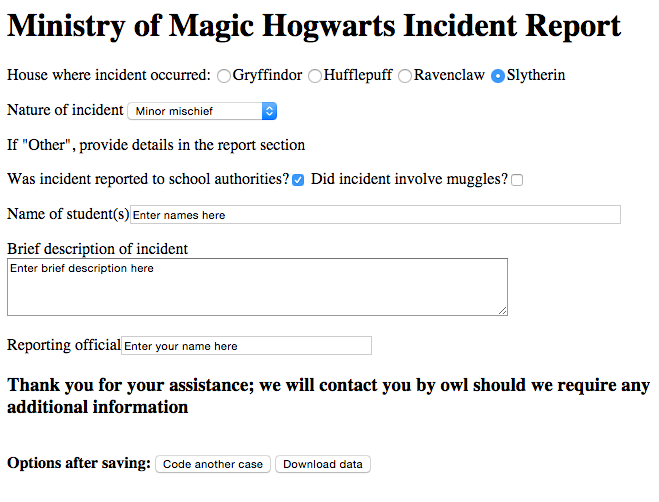
\includegraphics{demo_template.png}
\end{figure}


\chapter{Appendix 2: Input Format}
\label{appendix2:appendix-2-input-format}\label{appendix2::doc}
Fields marked with ** are required. Text fields are limited to 100 characters except
for:
\begin{itemize}
\item {} 
\code{textoriginal}, \code{textmkup} and \code{casevalues} have no length limitation

\item {} 
the three comment fields \code{collcmt}, \code{textcmt} and \code{casecmt} can be up
to 500 characters

\item {} 
coder ID, which is limited to 32 characters.

\end{itemize}


\section{Collection fields}
\label{appendix2:collection-fields}\begin{description}
\item[{collid}] \leavevmode
Collection ID, which needs to be unique within the workspace. If
this is not provided in the file, collfilename is assigned by the
program

\item[{collfilename}] \leavevmode
directory and name of the YAML file (without the suffix) where the
file was read from; this is assigned by the program

\item[{colldate}] \leavevmode
collection date YYYY-MM-DD

\item[{**colledit}] \leavevmode
datetime of editing of this collection  {[}provided by system{]}

\item[{collcmt}] \leavevmode
collection comments

\item[{categories {[}optional{]}}] \leavevmode
categories and items for dynamic selection menus (\textbf{dynselect})

\item[{texts}] \leavevmode
one or more related texts

\item[{cases}] \leavevmode
zero or more coded records

\end{description}


\section{Category fields}
\label{appendix2:category-fields}
These are all indented: the first line is the category name followed by a required colon (:). This is followed by the
menu options, one per line preceded by an indent and a hyphen-space (\code{- {}`{}`). If the menu option begins with an asterisk (}*{}`{}`)
it is the default value for the menu.  The following figure shows an example of menu items specified for three categories,
\code{statecat},{}`{}`torgcat{}`{}` and \code{loccat.}
\begin{figure}[htbp]
\centering

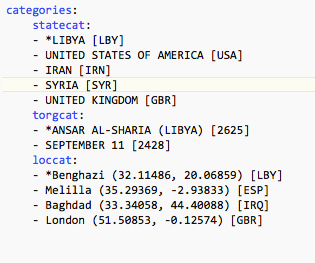
\includegraphics{category_example.png}
\end{figure}


\section{Text fields}
\label{appendix2:text-fields}\begin{description}
\item[{**textid}] \leavevmode
unique text ID for CIVET. This needs to be unique within the
workspace, and given how collections might get mixed across
workspace folders, ideally should be unique for the entire project.
If a value for the \code{text} field is not provided it will be
assigned by the program.

\item[{**textdate}] \leavevmode
text date YYYY-MM-DD

\item[{textdelete:}] \leavevmode
Boolean: text has been marked for deletion.

\item[{textpublisher}] \leavevmode
publisher {[}any string{]}

\item[{textpubid}] \leavevmode
publisher ID {[}any string{]}

\item[{textbiblio}] \leavevmode
bibliographic citation

\item[{textgeogloc}] \leavevmode
geographical locations

\item[{textauthorr}] \leavevmode
author {[}any string{]}

\item[{textlang}] \leavevmode
language

\item[{textlicense}] \leavevmode
copyright notification or other license information

\item[{**textlede}] \leavevmode
lede/headline/abstract—this is a short summary of the article
which will be highlighted and also will appear in the sorting
routine.

\item[{textcmt}] \leavevmode
comment

\item[{**textoriginal}] \leavevmode
original text of the story; this will not be modified by the system

\item[{textmkup}] \leavevmode
marked up text: this is the annotated version of the story with
any mark-up that has been added either automatically on manually

\item[{textmkupdate}] \leavevmode
datetime time of editing of this block {[}provided by system{]}

\item[{textmkupcoder}] \leavevmode
coder ID

\end{description}


\section{Case fields}
\label{appendix2:case-fields}\begin{description}
\item[{** caseid}] \leavevmode
Internal case/event ID. This is assigned by the program and
probably should not be changed; external IDs can be entered as
variables.

\item[{** casedate}] \leavevmode
Date and time this case was coded {[}provided by system{]}

\item[{casecmt}] \leavevmode
comment for case

\item[{casecoder}] \leavevmode
coder ID

\item[{casevalues}] \leavevmode
This is a string formatted as a Python dictionary which contains
pairs of variable names and values

\end{description}


\section{Date formats}
\label{appendix2:date-formats}
{[}This has not been consistently implemented in Beta-0.9{]}

Dates are ISO-8601 (\href{http://en.wikipedia.org/wiki/ISO\_8601}{http://en.wikipedia.org/wiki/ISO\_8601};
\href{http://www.w3.org/TR/NOTE-datetime}{http://www.w3.org/TR/NOTE-datetime}; \href{https://xkcd.com/1179/}{https://xkcd.com/1179/};
\href{http://www.cl.cam.ac.uk/mgk25/iso-time.html}{http://www.cl.cam.ac.uk/mgk25/iso-time.html}) so generally either
\begin{itemize}
\item {} 
YYYY-MM-DD

\item {} 
YYYY-MM-DDThh:mm:ss

\item {} 
YYYY-MM-DDThh:mm:ss{[}+-{]}hh:mm

\end{itemize}


\section{UTF-8 Encodings}
\label{appendix2:utf-8-encodings}
The system currently translates \href{https://en.wikipedia.org/wiki/UTF-8}{UTF-8}
encodings to \href{https://en.wikipedia.org/wiki/ASCII}{ASCII} using the
Django function \code{encoding.smart\_str()}. We expect to eventually
convert CIVET to Python 3.x (at present it is Python 2.7) which
is UTF-8 “native” but it isn't there yet, so you are best off doing
your own conversions during the process of converting the original
texts to the YAML formatting.


\section{Sample File}
\label{appendix2:sample-file}
The following figure shows an example of a simple YAML file; This is a screen capture of a file being edited with \emph{BBEdit},
hence the color mark-up. A workspace demonstration file with several collections can also be downloaded in the program.
\begin{figure}[htbp]
\centering

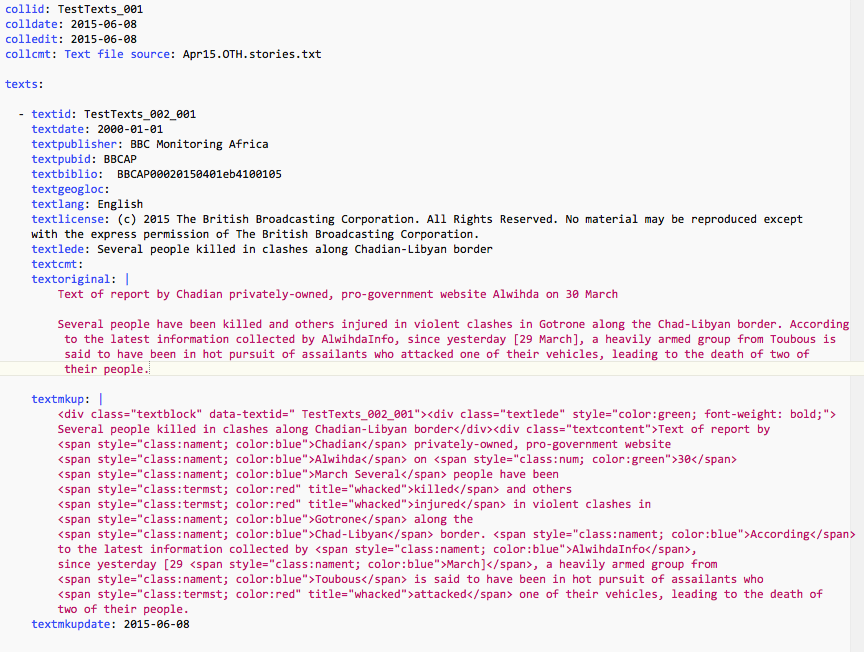
\includegraphics{yamlexample.png}
\end{figure}


\chapter{Appendix 3: Supporting Files and Source Code Settings}
\label{appendix3:appendix-3-supporting-files-and-source-code-settings}\label{appendix3::doc}

\section{Files in \texttt{/static/djciv\_data}}
\label{appendix3:files-in-static-djciv-data}

\subsection{Files that can be modified using a text editor}
\label{appendix3:files-that-can-be-modified-using-a-text-editor}\begin{description}
\item[{CIVET.demo.template.txt:}] \leavevmode
Demonstration template file for simple coding

\item[{CIVET.workspace.demo.zip:}] \leavevmode
Demonstration workspace with sample collections, coding form and
user-specified coding categories

\item[{CIVET.stopwords.txt:}] \leavevmode
Stop words for automatic named-entity annotation

\item[{CIVET.numberwords.txt:}] \leavevmode
Number words and phrases for automatic number annotation

\end{description}


\subsection{Modify at your own risk}
\label{appendix3:modify-at-your-own-risk}\begin{description}
\item[{ckeditor:}] \leavevmode
This is a “CKEditor” file downloaded from
\href{http://ckeditor.com/}{http://ckeditor.com/}: if you would like additional features you
should be able to create your own and swap it in here.

\end{description}


\subsection{CIVET Logo}
\label{appendix3:civet-logo}\begin{description}
\item[{civet\_logo.png:}] \leavevmode
Don’t like our little guy, or want to put your own mascot here?—this
is the place to make the change

\end{description}


\section{Additional settings that can be changed in \texttt{civet\_settings.py}}
\label{appendix3:additional-settings-that-can-be-changed-in-civet-settings-py}
These are global options but do not appear in the “Preferences” menu since there
is little reason to change them dynamically (and usually plenty of reasons not to)
\begin{description}
\item[{\textbf{Hide ‘Read coding form’}}] \leavevmode
Hide the ‘Read coding form’ button on the home screen: this can be used if you
only intend coders to be using workspaces.
\begin{itemize}
\item {} 
Default: \code{False}

\item {} 
\textbf{civet\_settings.py} variable: \code{HIDE\_READ\_CODING\_FORM}

\end{itemize}

\item[{\textbf{Hide ‘Read workspace’}}] \leavevmode
Hide the ‘Read workspace’ button on the home screen: this can be used if you
only intend coders to be using coding forms.
\begin{itemize}
\item {} 
Default: \code{False}

\item {} 
\textbf{civet\_settings.py} variable: \code{HIDE\_READ\_WORKSPACE}

\end{itemize}

\item[{\textbf{Hide ‘Preferences’}}] \leavevmode
Hide the ‘Preferences’ button on the home screen: this can be used if you
don't want coders changing these.
\begin{itemize}
\item {} 
Default: \code{False}

\item {} 
\textbf{civet\_settings.py} variable: \code{HIDE\_PREFERENCES}

\end{itemize}

\end{description}


\section{Documentation}
\label{appendix3:documentation}
CIVET's documentation is maintained using the Sphinx \href{http://sphinx-doc.org/}{http://sphinx-doc.org/} system.
The files are found in the \code{docs} directory at the outer-most level of the system.
The commands:

\begin{Verbatim}[commandchars=\\\{\}]
make html
make latexpdf
\end{Verbatim}

are used to generate the on-line and PDF documentation; the files are found in the
\code{\_build/html} and \code{\_build/latex} directories.

Because of the images and the redundant files in the “\_build” directory,
“djcivet\_site/docs” is a very large directory, about 70\% of the size of the
full “djcivet\_site” directory, and can be removed in deployments where you are
just planning to use the on-line documentation. In that situation, the roughly 1 Mb file
“djcivet\_site/djciv\_data/static/djciv\_data/civdocs.pdf” can also be removed,
to the code for the system itself is only about 2 Mb.


\chapter{Appendix 4: Prototype on Google Application Engine}
\label{appendix4:appendix-4-prototype-on-google-application-engine}\label{appendix4::doc}
An earlier demonstration version of the program, written in the Flask
\href{http://flask.pocoo.org/}{http://flask.pocoo.org/} micro-framework , is deployed as an application on the Google App Engine at
\href{http://ace-element-88313.appspot.com/}{http://ace-element-88313.appspot.com/}.  The code
for this version can be downloaded from \href{https://github.com/philip-schrodt/CIVET-Flask}{https://github.com/philip-schrodt/CIVET-Flask}.
The Flask version has most of the data entry commands, but none of the
workspace commands.

The other option in the program is the “Text-Extraction Demonstration
Form” which was a prototype of the full annotation/extraction system. To
activate the demo, from the home page, click the link in the line \emph{See a
demo of the text-highlighting system by clicking here}
\begin{enumerate}
\item {} 
Select a text file to edit: you can use either the pull-down menu or
radio boxes, then click the \code{Edit the file button}.

\item {} 
Click one of the text entry boxes will highlight the relevant words
in text: For demonstration purposes these are words beginning with
the letters ’a’, ’c’, ’d’, ’e’ and ’s’. The ‘tab’ key cycles between
these options, or an option can be selected using the mouse.

\item {} 
When a text entry box is active, the first relevant word in the text
is highlighted. The right-arrow key will cycle the highlighted word.
To copy a highlighted word into the text box, use the down-arrow key.

\item {} 
Text can also be selected using the mouse: To copy the selected text
into the text box, use the left-arrow key.

\item {} 
Cut-and-paste from the text to the date fields work as you would
expect

\item {} 
Text can also be entered manually.

\item {} 
To save a set of coded fields, click one of the buttons along the
bottom.
\begin{description}
\item[{Return to this case:}] \leavevmode
Save, then return to the same text

\item[{Select new case:}] \leavevmode
Save, then return to the same text

\item[{Download data:}] \leavevmode
Save, then download data as a text file

\end{description}

\item {} 
The ``CIVET Download'' page provides a text box for a file name, and
the \code{Download file} button downloads the coded data. Use the \emph{Start
new data file} link to re-start the coding and the \emph{Continue coding
with this file} link to continue adding to the existing records.
\begin{itemize}
\item {} 
The .txt file contains the variable names in the first line.

\item {} 
If the file name does not end in ''.txt'', this will be
added.

\end{itemize}

\item {} 
To quit the program, just close the window: This is a HTML/Javascript security feature which
prevents rogue websites from closing windows unless they have created
the window.

\end{enumerate}

If you don't need the content management or extraction facilities of CIVET
workspaces, Flask is simpler and easier to deploy than Django, but has much
the same model-view-controller logical structure, and like Django uses the
“jinja2” template system for web pages. It should be relatively
straightforward to retro-fit the new features of the forms system—notably
the “//” and “/” prefixes—to the older code.



\renewcommand{\indexname}{Index}
\printindex
\end{document}
